%%%%%%%%%%%%%%%%%%%%%%%%%%%%%%%%%%%%%%%%%
% Short Sectioned Assignment
% LaTeX Template
% Version 1.0 (5/5/12)
%
% This template has been downloaded from:
% http://www.LaTeXTemplates.com
%
% Original author:
% Frits Wenneker (http://www.howtotex.com)
%
% License:
% CC BY-NC-SA 3.0 (http://creativecommons.org/licenses/by-nc-sa/3.0/)
%
%%%%%%%%%%%%%%%%%%%%%%%%%%%%%%%%%%%%%%%%%

%----------------------------------------------------------------------------------------
%	PACKAGES AND OTHER DOCUMENT CONFIGURATIONS
%----------------------------------------------------------------------------------------

\documentclass[paper=a4, fontsize=12pt]{scrartcl} % A4 paper and 11pt font size

\usepackage[T1]{fontenc} % Use 8-bit encoding that has 256 glyphs
\usepackage{fourier} % Use the Adobe Utopia font for the document - comment this line to return to the LaTeX default
\usepackage[english]{babel} % English language/hyphenation
\usepackage{amsmath,amsfonts,amsthm} % Math packages

\usepackage{sectsty} % Allows customizing section commands
\allsectionsfont{\centering \normalfont\scshape} % Make all sections centered, the default font and small caps

\usepackage{graphicx}

\usepackage[a4paper,lmargin=2.5 cm,rmargin=2 cm,tmargin=2 cm,bmargin=2 cm]{geometry}

\usepackage{fancyhdr} % Custom headers and footers
\pagestyle{fancyplain} % Makes all pages in the document conform to the custom headers and footers
\fancyhead{} % No page header - if you want one, create it in the same way as the footers below
\fancyfoot[L]{} % Empty left footer
\fancyfoot[C]{} % Empty center footer
\fancyfoot[C]{\thepage} % Page numbering for right footer
\renewcommand{\headrulewidth}{0pt} % Remove header underlines
\renewcommand{\footrulewidth}{0pt} % Remove footer underlines
\setlength{\headheight}{13.6pt} % Customize the height of the header

\usepackage{chngcntr}
%\numberwithin{equation}{section} % Number equations within sections (i.e. 1.1, 1.2, 2.1, 2.2 instead of 1, 2, 3, 4)
%\numberwithin{figure}{section} % Number figures within sections (i.e. 1.1, 1.2, 2.1, 2.2 instead of 1, 2, 3, 4)
%\counterwithout{figure}{section}
%\numberwithin{table}{section} % Number tables within sections (i.e. 1.1, 1.2, 2.1, 2.2 instead of 1, 2, 3, 4)

\setlength\parindent{0pt} % Removes all indentation from paragraphs - comment this line for an assignment with lots of text

\usepackage{amsmath}
\usepackage{float} % To firce the location of figure
\usepackage{subfigure} %For side-by-side figures
\usepackage{lettrine}
%\usepackage{lipsum}
\usepackage{epstopdf} %To read *.eps Files
\usepackage{listings} % To include source codes in LATEX document
\usepackage{mathrsfs} % To include script fonts. use \mathscr{}
\usepackage{courier} % To write in courier fornt
\usepackage{mathtools} % For mat symbols
\usepackage{xfrac} % For \sfrac{}{}
%----------------------------------------------------------------------------------------
%	TITLE SECTION
%----------------------------------------------------------------------------------------

\newcommand{\horrule}[1]{\rule{\linewidth}{#1}} % Create horizontal rule command with 1 argument of height

\title{	
\normalfont \normalsize 
\textsc{Wright State University\\ Department of Mechanical and Materials Engineering} \\ [25pt] % Your university, school and/or department name(s)
\horrule{0.5pt} \\[0.4cm] % Thin top horizontal rule
\LARGE ME7060 - Structural Reliability \\ % The assignment title
\LARGE Fluid-Solid Interaction Based Reliability Analysis \\
\Large Project Report
\horrule{2pt} \\[0.5cm] % Thick bottom horizontal rule
}

\usepackage{setspace}
\doublespacing

\author{Koorosh Gobal} % Your name

\date{\normalsize\today} % Today's date or a custom date

\begin{document}

\maketitle % Print the title

%----------------------------------------------------------------------------------------
%	PROBLEM 1
%----------------------------------------------------------------------------------------
\section{Scope of Work}
The coupling between the fluid and structure response has always been an interesting problem for the aerospace researchers. Many aerospace structures undergo loading scenarios that are affected from both the solid and fluids domain. The aerodynamic loads on a wing for example, are generated due to the pressure gradients around the wing body. These forces are conveyed to the fuselage by the wing structure to maintain a lift force required for the aircraft to continue its flight path. The wing structure deforms due to the aerodynamic loads causing its angle of the attack (AoA) to change. It is well known that one of the contributing factors on the flow field around wings is the AoA of the wing airfoil. Therefore, change in AoA causes the flow field to change and this requires the aerodynamic forces to be updated. A two-way coupling is needed between the flow field and the structure to capture the true effects of the interactions between the two physics.\\

In this project we have investigated the effect of uncertainties on the robustness of simple wing structure to main the required lift force. The lift force is one of the most crucial parameters in the design and safety of an aircraft. The uncertainties are included both in the flow field and the wing structure. These will discussed in more detail in the following sections. The most important part of this project is development of a two-way coupling between a computational fluid dynamic (CFD) and finite element analysis (FEA) solver. \emph{OpenFOAM} is chosen as the CFD solver for this project and is coupled with \emph{fem4d} FEA solver developed by CEPRO research group. The two solvers are coupled in Matlab on a LINUX machine. Matlab handled transferring the data between the two solvers and updating the models. Moreover, Matlab is responsible for running UQ simulations. In this project First Order Reliability Method (FORM) is used to calculate the reliability index of the limit-state function (lift force). Function approximation technique (TANA) is used to solve the optimization problem of calculating the reliability index. Finally convolution theorem is used to demonstrate the shape of the distribution of the limit-state function.\\

As a comparison between this project and homework problems, it can be argued that the simulation part of this project is much more complicated than the homework problems. This is due to the fact that many iterations between two solvers is required to get a converged solution. Transferring loads from the CFD to FEA solver and sending the displacement data back to modify the shape of the fluids domain is another factor that adds to the complexity of the problem. Moreover in this project different probability density functions are used which requires additional step of transferring them to the equivalent normal distribution. This has not been touched in the homework problems as well.
%----------------------------------------------------------------------------------------
%	PROBLEM 1
%----------------------------------------------------------------------------------------
\section{Problem Formulation}\label{sec:problemFormulation}
%----------------------------------------------------------------------------------------
Fluid-structure interaction (FSI) is the interaction of some movable or deformable structure with an internal or surrounding fluid flow. Fluid-structure interactions are a crucial consideration in the design of many engineering systems, e.g. aircraft and bridges. Tacoma Narrows Bridge (1940), is probably one of the most infamous examples of large-scale failure.\\

Fluid-structure interaction problems and multiphysics problems in general are often too complex to solve analytically and so they have to be analyzed by means of experiments or numerical simulation. Two main approaches exist for the simulation of fluid-structure interaction problems:
%
\begin{itemize}
	\item Monolithic approach: the equations governing the flow and the 
		displacement of the structure are solved simultaneously, with a single 
		solver.
	\item Partitioned approach: the equations governing the flow and the 
		displacement of the structure are solved separately, with two distinct 
		solvers.
\end{itemize}
%
The monolithic approach requires a code developed for this particular combination of physical problems whereas the partitioned approach preserves software modularity because an existing flow solver and structural solver are coupled. Moreover, the partitioned approach facilitates solution of the flow equations and the structural equations with different, possibly more efficient techniques which have been developed specifically for either flow equations or structural equations. On the other hand, development of stable and accurate coupling algorithm is required in partitioned simulations.\\

In this project the partitioned approach have been chosen due to its simplicity to implement and availability of separate CFD and FEA solvers. The simplified geometry of a wing used in this project is shown in Figure ~\ref{fig:model_geometery}. As shown in this figure, the wing is modeled as an airfoil that is connected to the tip of a beam. The airfoil represents the lifting surfaces whereas the beam models the wing structure. The Boeing airfoil J is used as the airfoil model. This is the same airfoil that 747 Boeing aircraft uses in its wings. The aerodynamic forces acting on the airfoil are transferred to the structure through the connection point.\\
%
\begin{figure}[H]
	\centering
	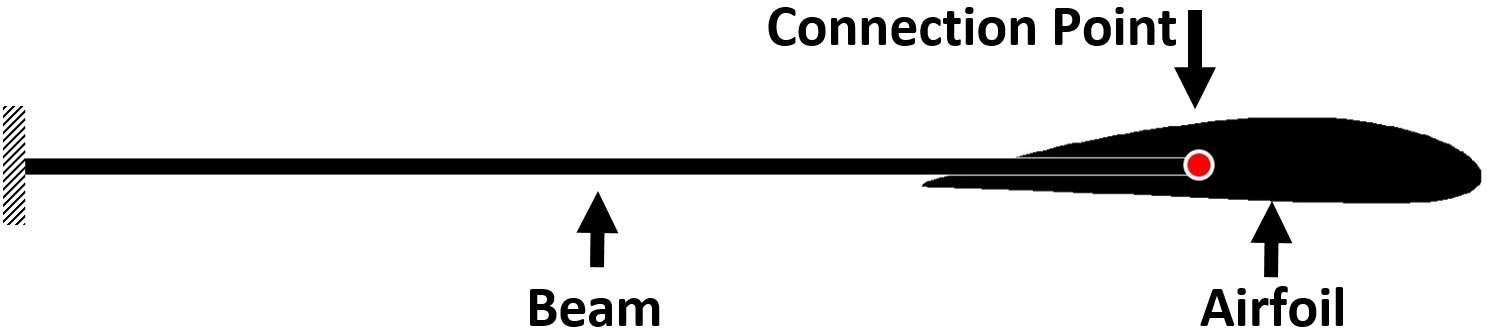
\includegraphics[height=2.5cm]{model_geometery.jpg}
	\caption{Simplified model of a wing.}
	\label{fig:model_geometery}
\end{figure}
%
The CFD model is shown in Figure ~\ref{fig:CFDmodel}. The boundary conditions are applied as constant velocity with zero pressure gradient at the input and atmospheric pressure and zero velocity gradient at the output. It is assumed that the length of the domain is long enough so that the velocity profile won't change at the output of the model. Since the Reynolds number is large for this simulation (Re = 1.6571e+7) Spalart-Allmaras turbulence model is used as the simulation model \cite{spalart1997comments}. The pressure contour around the airfoil is shown in Figure ~\ref{fig:CFDresult} as the baseline simulation.\\
%
	\begin{figure}[H]
		\centering
		\subfigure[CFD domain.]
		{
		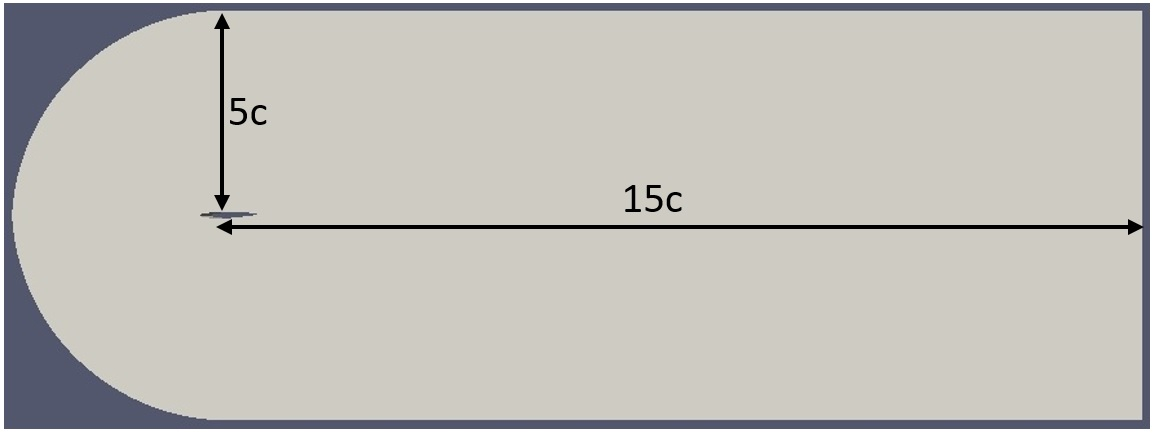
\includegraphics[height=5.15cm]{CFDdomain.jpg}
		\label{fig:CFDmodel}
		}
		\quad
		\subfigure[Bench mark result.]
		{
		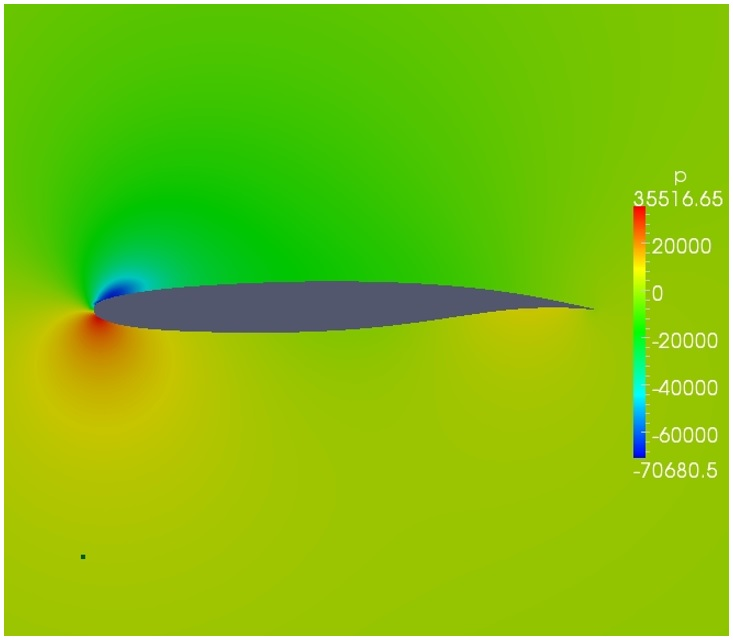
\includegraphics[height=5.15cm]{CFDresult.jpg}
		\label{fig:CFDresult}
		}
		\caption{CFD simulation.}
		\label{fig:random_variables_pdf}
	\end{figure}
%
The coupling procedure of fluid and structure is defined in the following lines as shown in the flow chart of Figure ~\ref{fig:FSI_simulation}:
%
\begin{itemize}
	\item The process starts by assigning the boundary conditions to the CFD problem and solving the flow field. The boundary condition that is effected by the coupling is the AoA. After solving the CFD problem, the pressure and velocity values are available at the mesh cells in the domain.

	\item Pressure data is sampled at the mesh cells on the airfoil surface. Coordinates for the mesh cells on the airfoil are used to define the discretized areas and their orientation. The orientation is needed to calculate the lift and drag forces. The pressure for each mesh cell is then used to calculate the corresponding force and its direction at each mesh cell on the airfoil. These force and moment are transferred to the structure using the connection point between the airfoil and the structure.

	\item The wing structure is modeled as a single beam element. The aerodynamic forces result in a deflection and rotation and the tip of the beam causing the AoA to change. The new AoA is sent to the CFD solver to update the aerodynamic loads. This process is repeated until the convergence is satisfied. The convergence criteria is selected as a threshold on change in AoA.
\end{itemize}
%
%
\begin{figure}[H]
	\centering
	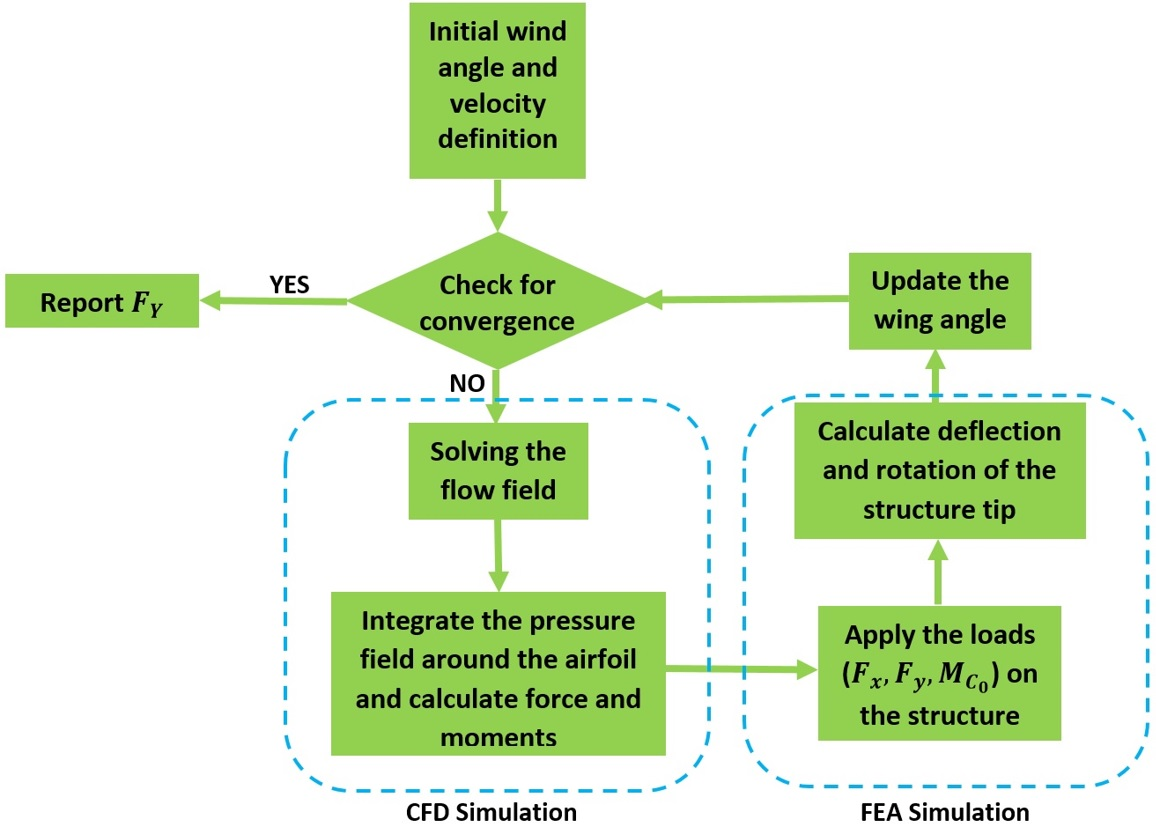
\includegraphics[height=10.75cm]{FSI_simulation.jpg}
	\caption{FSI coupling flow chart.}
	\label{fig:FSI_simulation}
\end{figure}
%
The above procedure can become unstable if the deflection at the first iteration becomes too large. To assure the stability of the solution, the beam deflection is relaxed so the AoA does not experience sudden changes. The sudden changes in AoA causes oscillation in the wing structure. The relaxation is done by letting the beam deflect less than the calculated value if the deflections become to large. The large deflection for this problem is defined as deflection larger than 5\% of the length of the beam. If the deflection exceeds this threshold, the deflection of 5\% is reported to calculate the AoA needed for the CFD solver. Using relaxation, we were able to achieve stability in the FSI simulation. The output of the FSI simulation is the lift force generated by the deflected wing structure. The output of system due to different input parameters is shown in Talbe ~\ref{table:resultsFSI}. As shown in this table, for most design cases the value of limit-state function is grater than zero. Therefore, it is expected to have low probability of failure.\\
%
\begin{table}[H]
\centering
\begin{tabular}{ c || c | c | c | c | c | c }
	Limit-state & U & $\alpha$ & $C_0$ & E & L & I \\
	\hline                       
	\hline
		8677.7 & 272.44 & 6.5171 & 0.44951 & 2.27E+11 & 1.1464 & 6.70E-07 \\
		3806.4 & 233.69 & 7.6384 & 0.58792 & 2.13E+11 & 1.0244 & 4.84E-07 \\
		17360 & 276.48 & 7.6257 & 0.40212 & 1.41E+11 & 1.0149 & 5.27E-07 \\
		1058 & 222.55 & 5.2702 & 0.47558 & 2.13E+11 & 1.1658 & 5.13E-07 \\
		7813.4 & 242.15 & 6.9399 & 0.36714 & 1.46E+11 & 0.91831 & 4.27E-07 \\
		1742.2 & 223.69 & 6.6702 & 0.52538 & 2.14E+11 & 1.0666 & 4.95E-07 \\
		8991.8 & 227.77 & 8.2554 & 0.37653 & 1.19E+11 & 1.0815 & 4.33E-07 \\
		14750 & 285.88 & 9.1865 & 0.45179 & 2.02E+11 & 0.97114 & 5.63E-07 \\
		14272 & 275.59 & 9.2185 & 0.50972 & 2.20E+11 & 1.0167 & 4.74E-07 \\
		2400 & 245.37 & 5.2727 & 0.56727 & 2.13E+11 & 0.8858 & 5.23E-07 \\
		18007 & 296.02 & 7.1547 & 0.58779 & 1.73E+11 & 0.88738 & 4.90E-07 \\
		52.377 & 222.76 & 4.5718 & 0.46416 & 1.89E+11 & 1.0055 & 5.34E-07 \\
		6653.9 & 255.1 & 4.773 & 0.34159 & 2.02E+11 & 1.0694 & 4.88E-07 \\
	\hline  
\end{tabular}
\caption{Fluid-structure interaction results.}
\label{table:resultsFSI}
\end{table}
%
The simulation is done on a LINUX machine with 3.4GHz processor and 16 GB of ram. Each full FSI simulation takes approximately 20 minutes to converge.
%----------------------------------------------------------------------------------------
%	PROBLEM 1
%----------------------------------------------------------------------------------------
\section{Reliability Information}
\subsection{Uncertain Variables}
Many uncertainties exist in the design of a wing structure for an aircraft. The uncertainties can exist in both the fluid and structure part of the model. In the fluid region velocity (U), wind angle ($\alpha$) are selected as the uncertain variables. On the other hand, for the structure part length of the wing (L), area moment of inertia (I), modulus of elasticity (E) and the connecting point between airfoil and the structure ($C_0$) are selected as uncertain variables. The location of connecting point is selected as a percentage of cord length from the tailing edge of the airfoil. It should be noted that changing the location of connection point affects the moment of load acting on the beam and as a result change the AoA and hence the lift force. As mentioned in Section ~\ref{sec:problemFormulation}, the limit-state for this problem is selected as the lift force generated by the wing. The wing must be capable of generating the required lift with the lowest probability of failure, i.e. not producing the required lift. The random variables and their distribution functions are shown in Table ~\ref{table:radom_variables}.
%
\begin{table}[H]
\centering
\begin{tabular}{ c | c | c | c }
	Random Variables & Distribution & \multicolumn{2}{|c}{Parameters} \\
	\hline                       
	\hline
		Wind velocity & Uniform & min = 220 & max = 300 \\
		Wind angle & Normal & $\mu = $ 7 & $\sigma = $ 2 \\
		Connection point & Uniform & min = 0.3 & max = 0.6 \\
		Elastic modulus & Weibull & $\lambda = $ 2E+11 & $k = $ 5 \\
		Length & Lognormal & $m = $ -0.0049752 & $v = $ 0.099751 \\
		Moment of inertia & Lognormal & $m = $ -14.474 & $v = $ 0.099751 \\
	\hline  
\end{tabular}
\caption{Random variables and their distributions.}
\label{table:radom_variables}
\end{table}
%
The Weibull distribution is assigned to the Elastic modulus. The reason for the selection is that the tail of the Weibull with shape parameter of 5 have zero probabilities. This is required when assigning the Elastic modulus since the elastic modulus cannot be infinity. The same reasoning is applicable for the chose of lognormal distribution. The lognormal distribution is always positive and can be applied to parameters that are required to have positive values such as length and moment of inertia of the beam. The probability distribution function (PDF) of the random variables is shown in Figure ~\ref{fig:random_variables_pdf}.
%
	\begin{figure}[H]
		\centering
		\subfigure[Velocity PDF.]
		{
		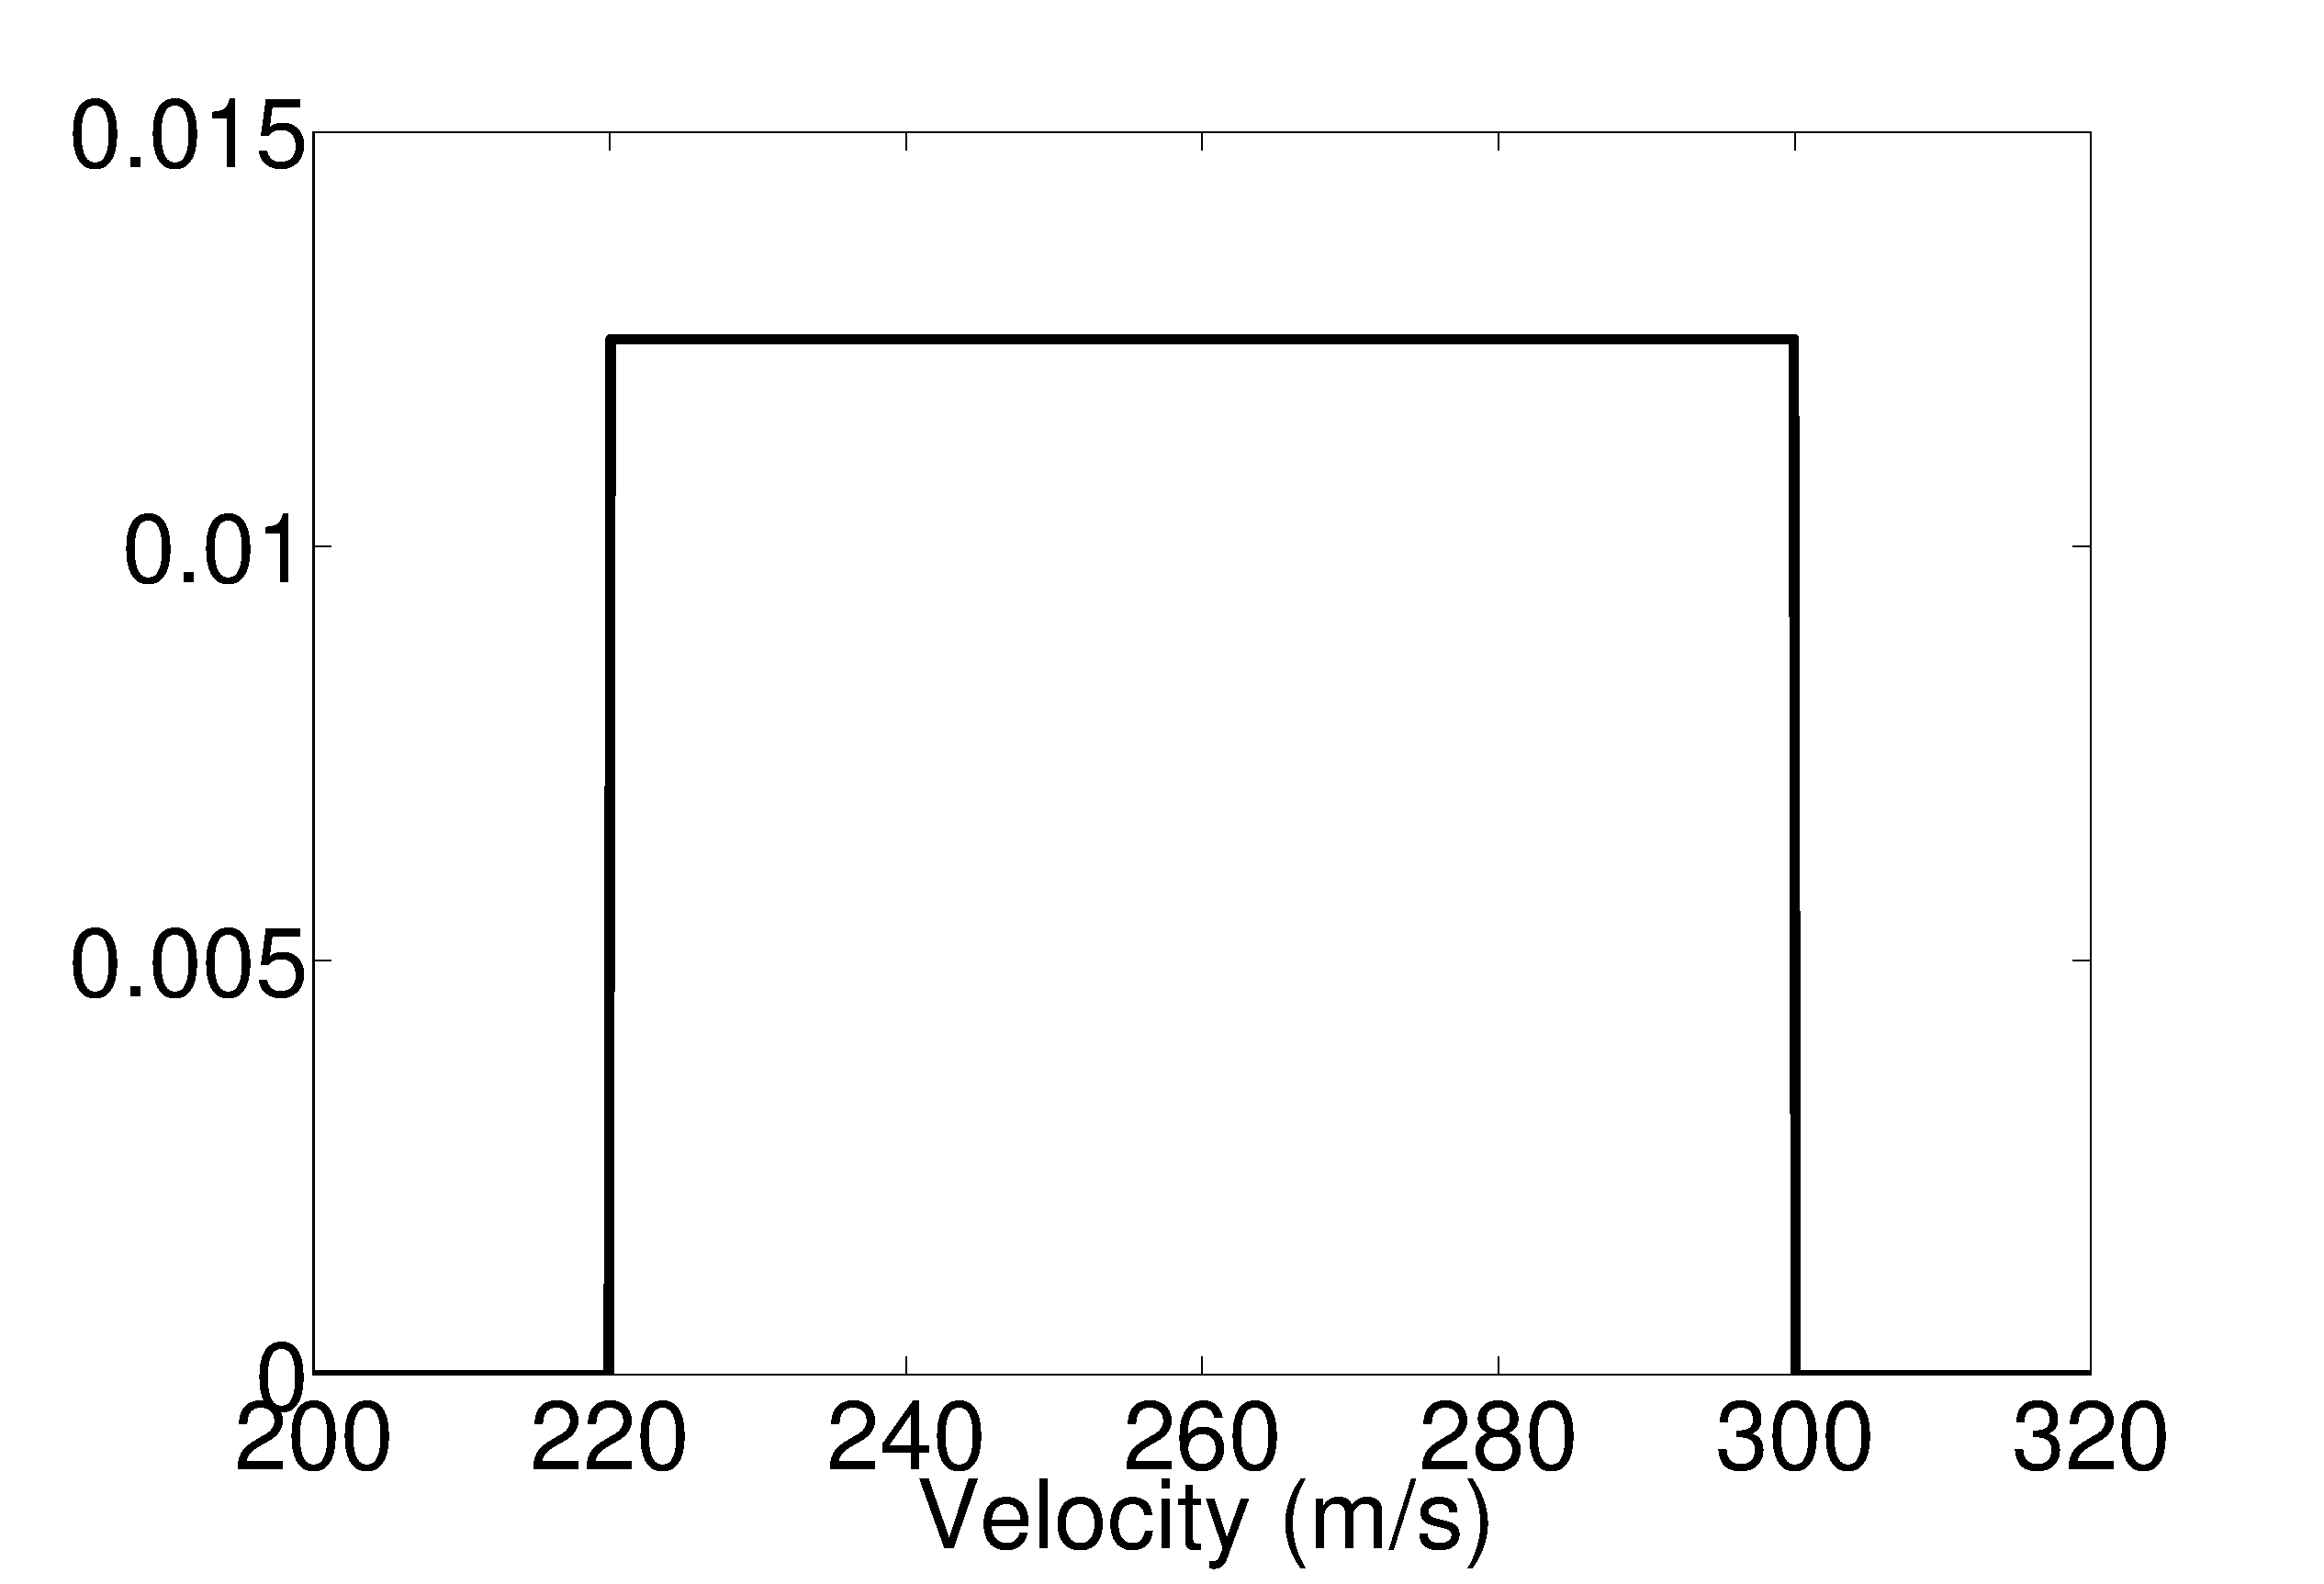
\includegraphics[height=5.15cm]{velocity_pdf.eps}
		\label{fig:results_fft}
		}
		\quad
		\subfigure[Wind angle PDF.]
		{
		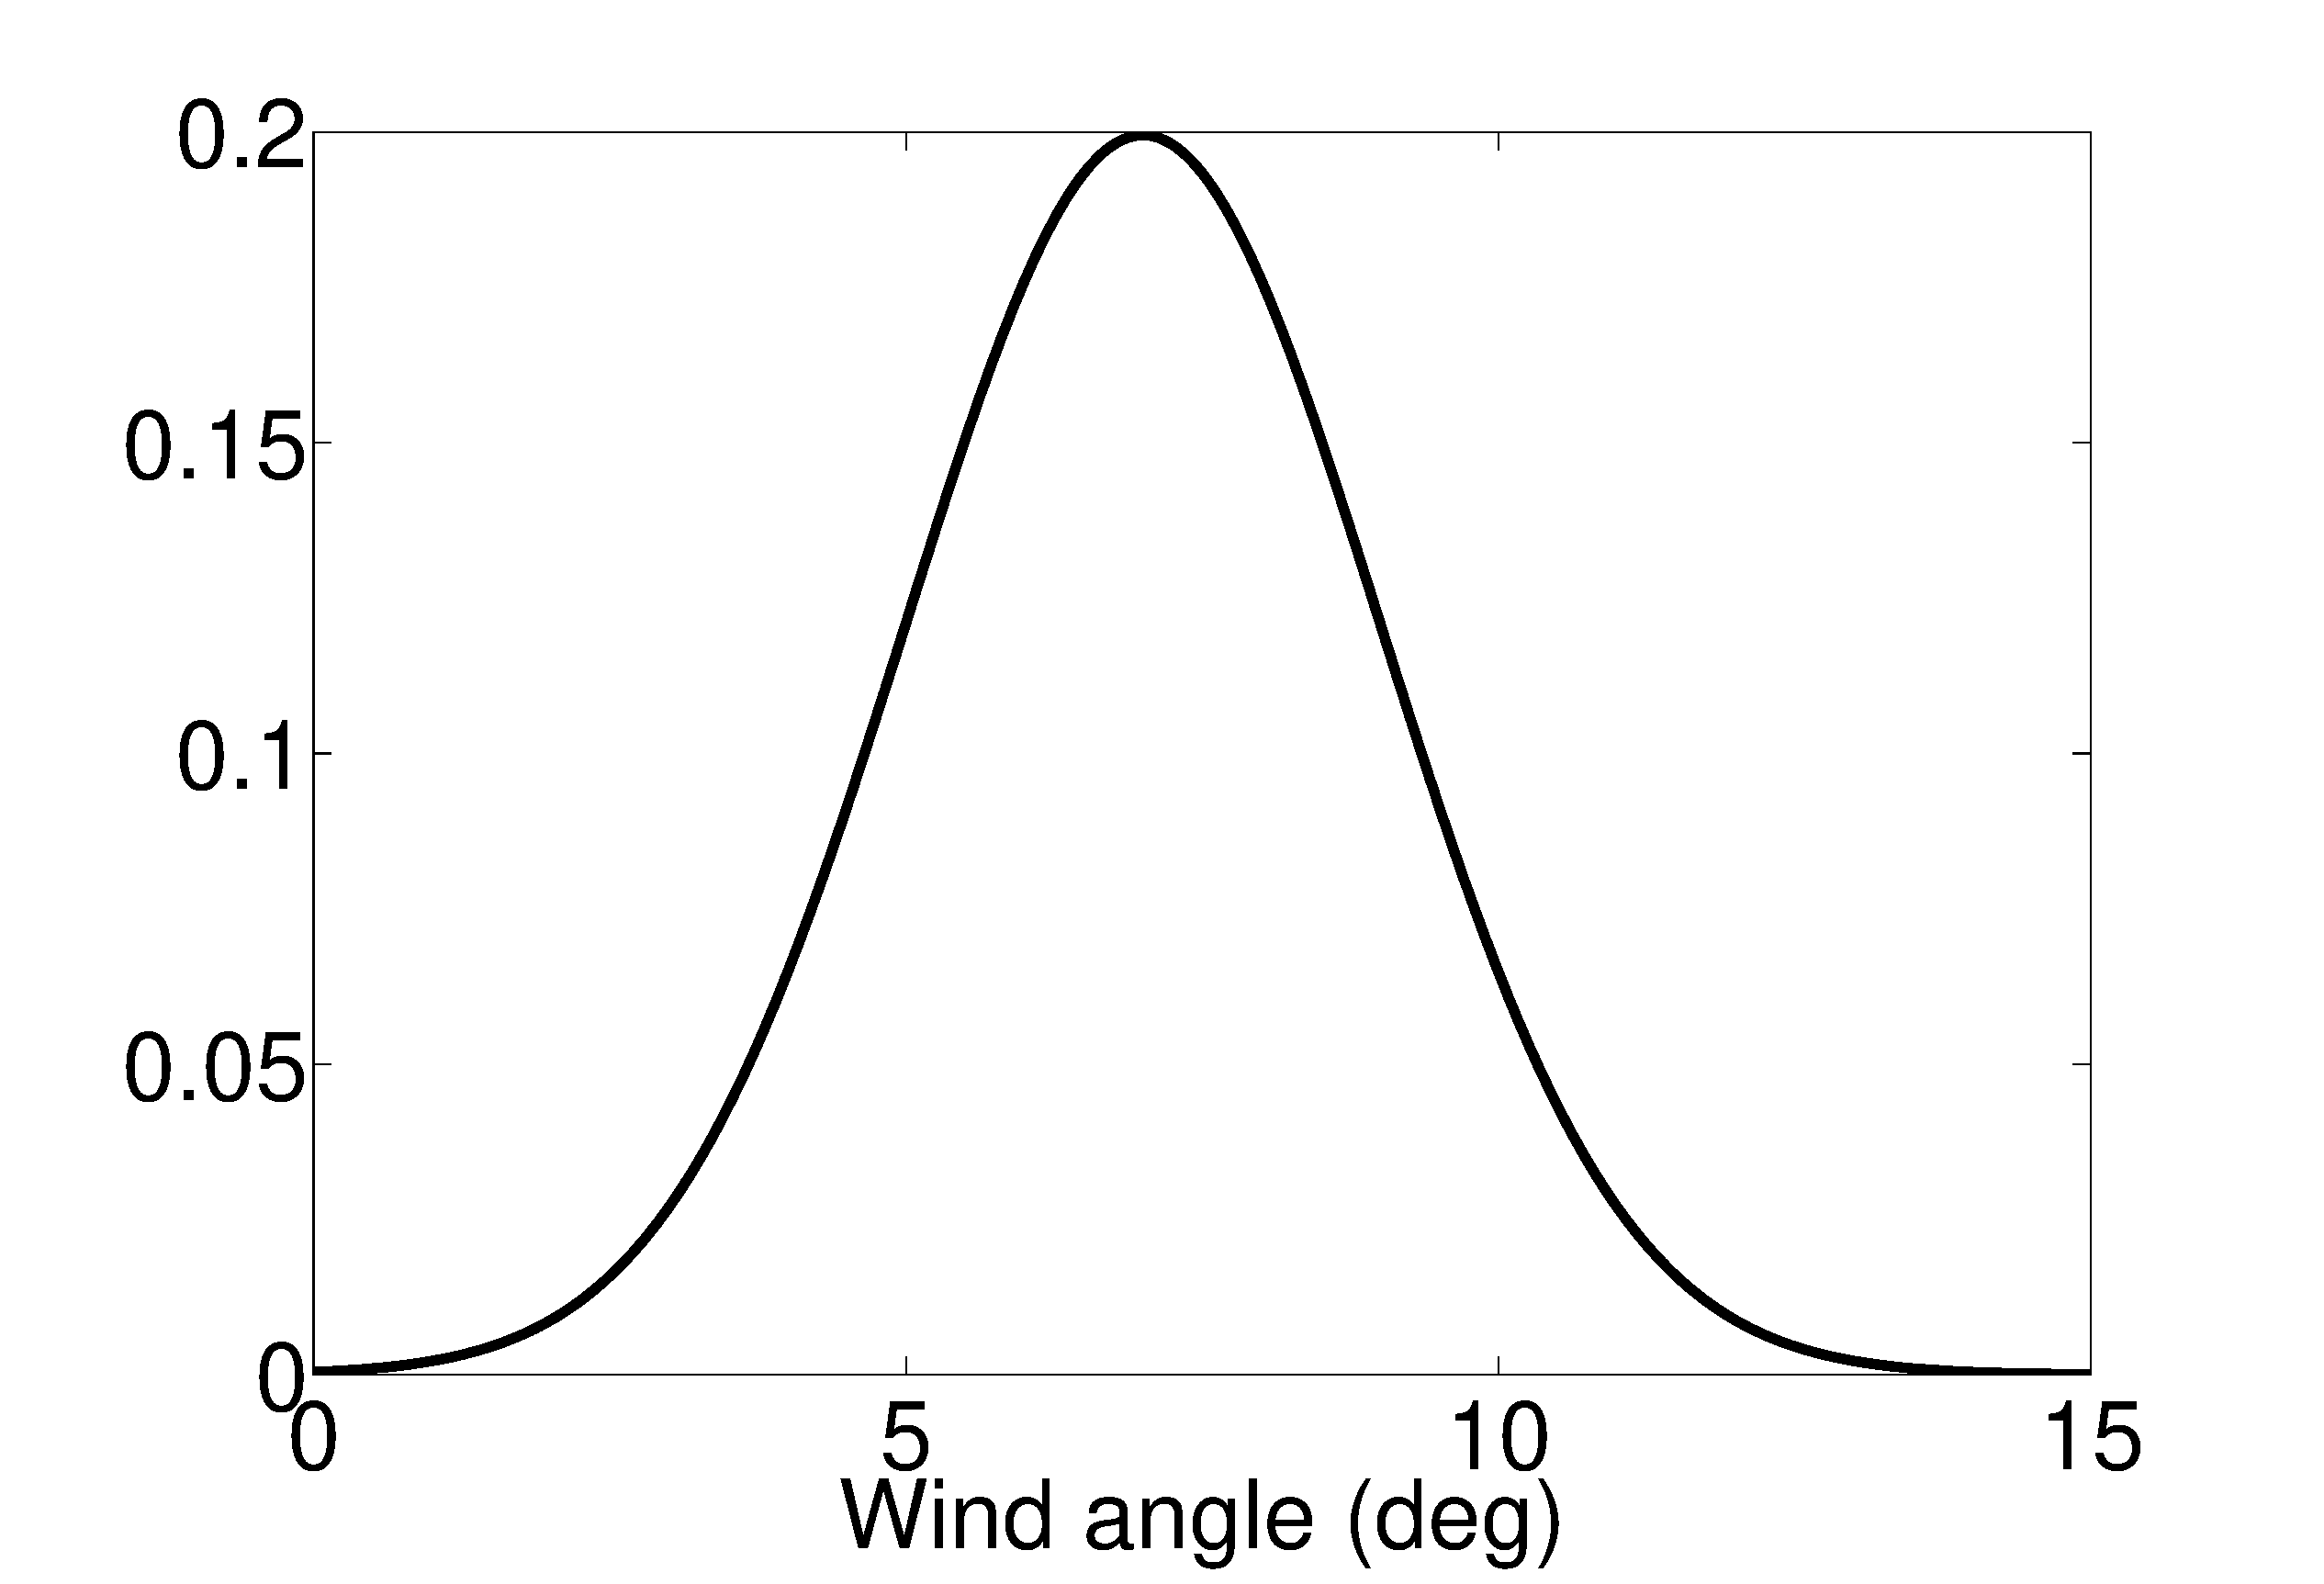
\includegraphics[height=5.15cm]{wind_angle_pdf.eps}
		\label{fig:results_hist}
		}
		\\
		\subfigure[Elastic modulus PDF.]
		{
		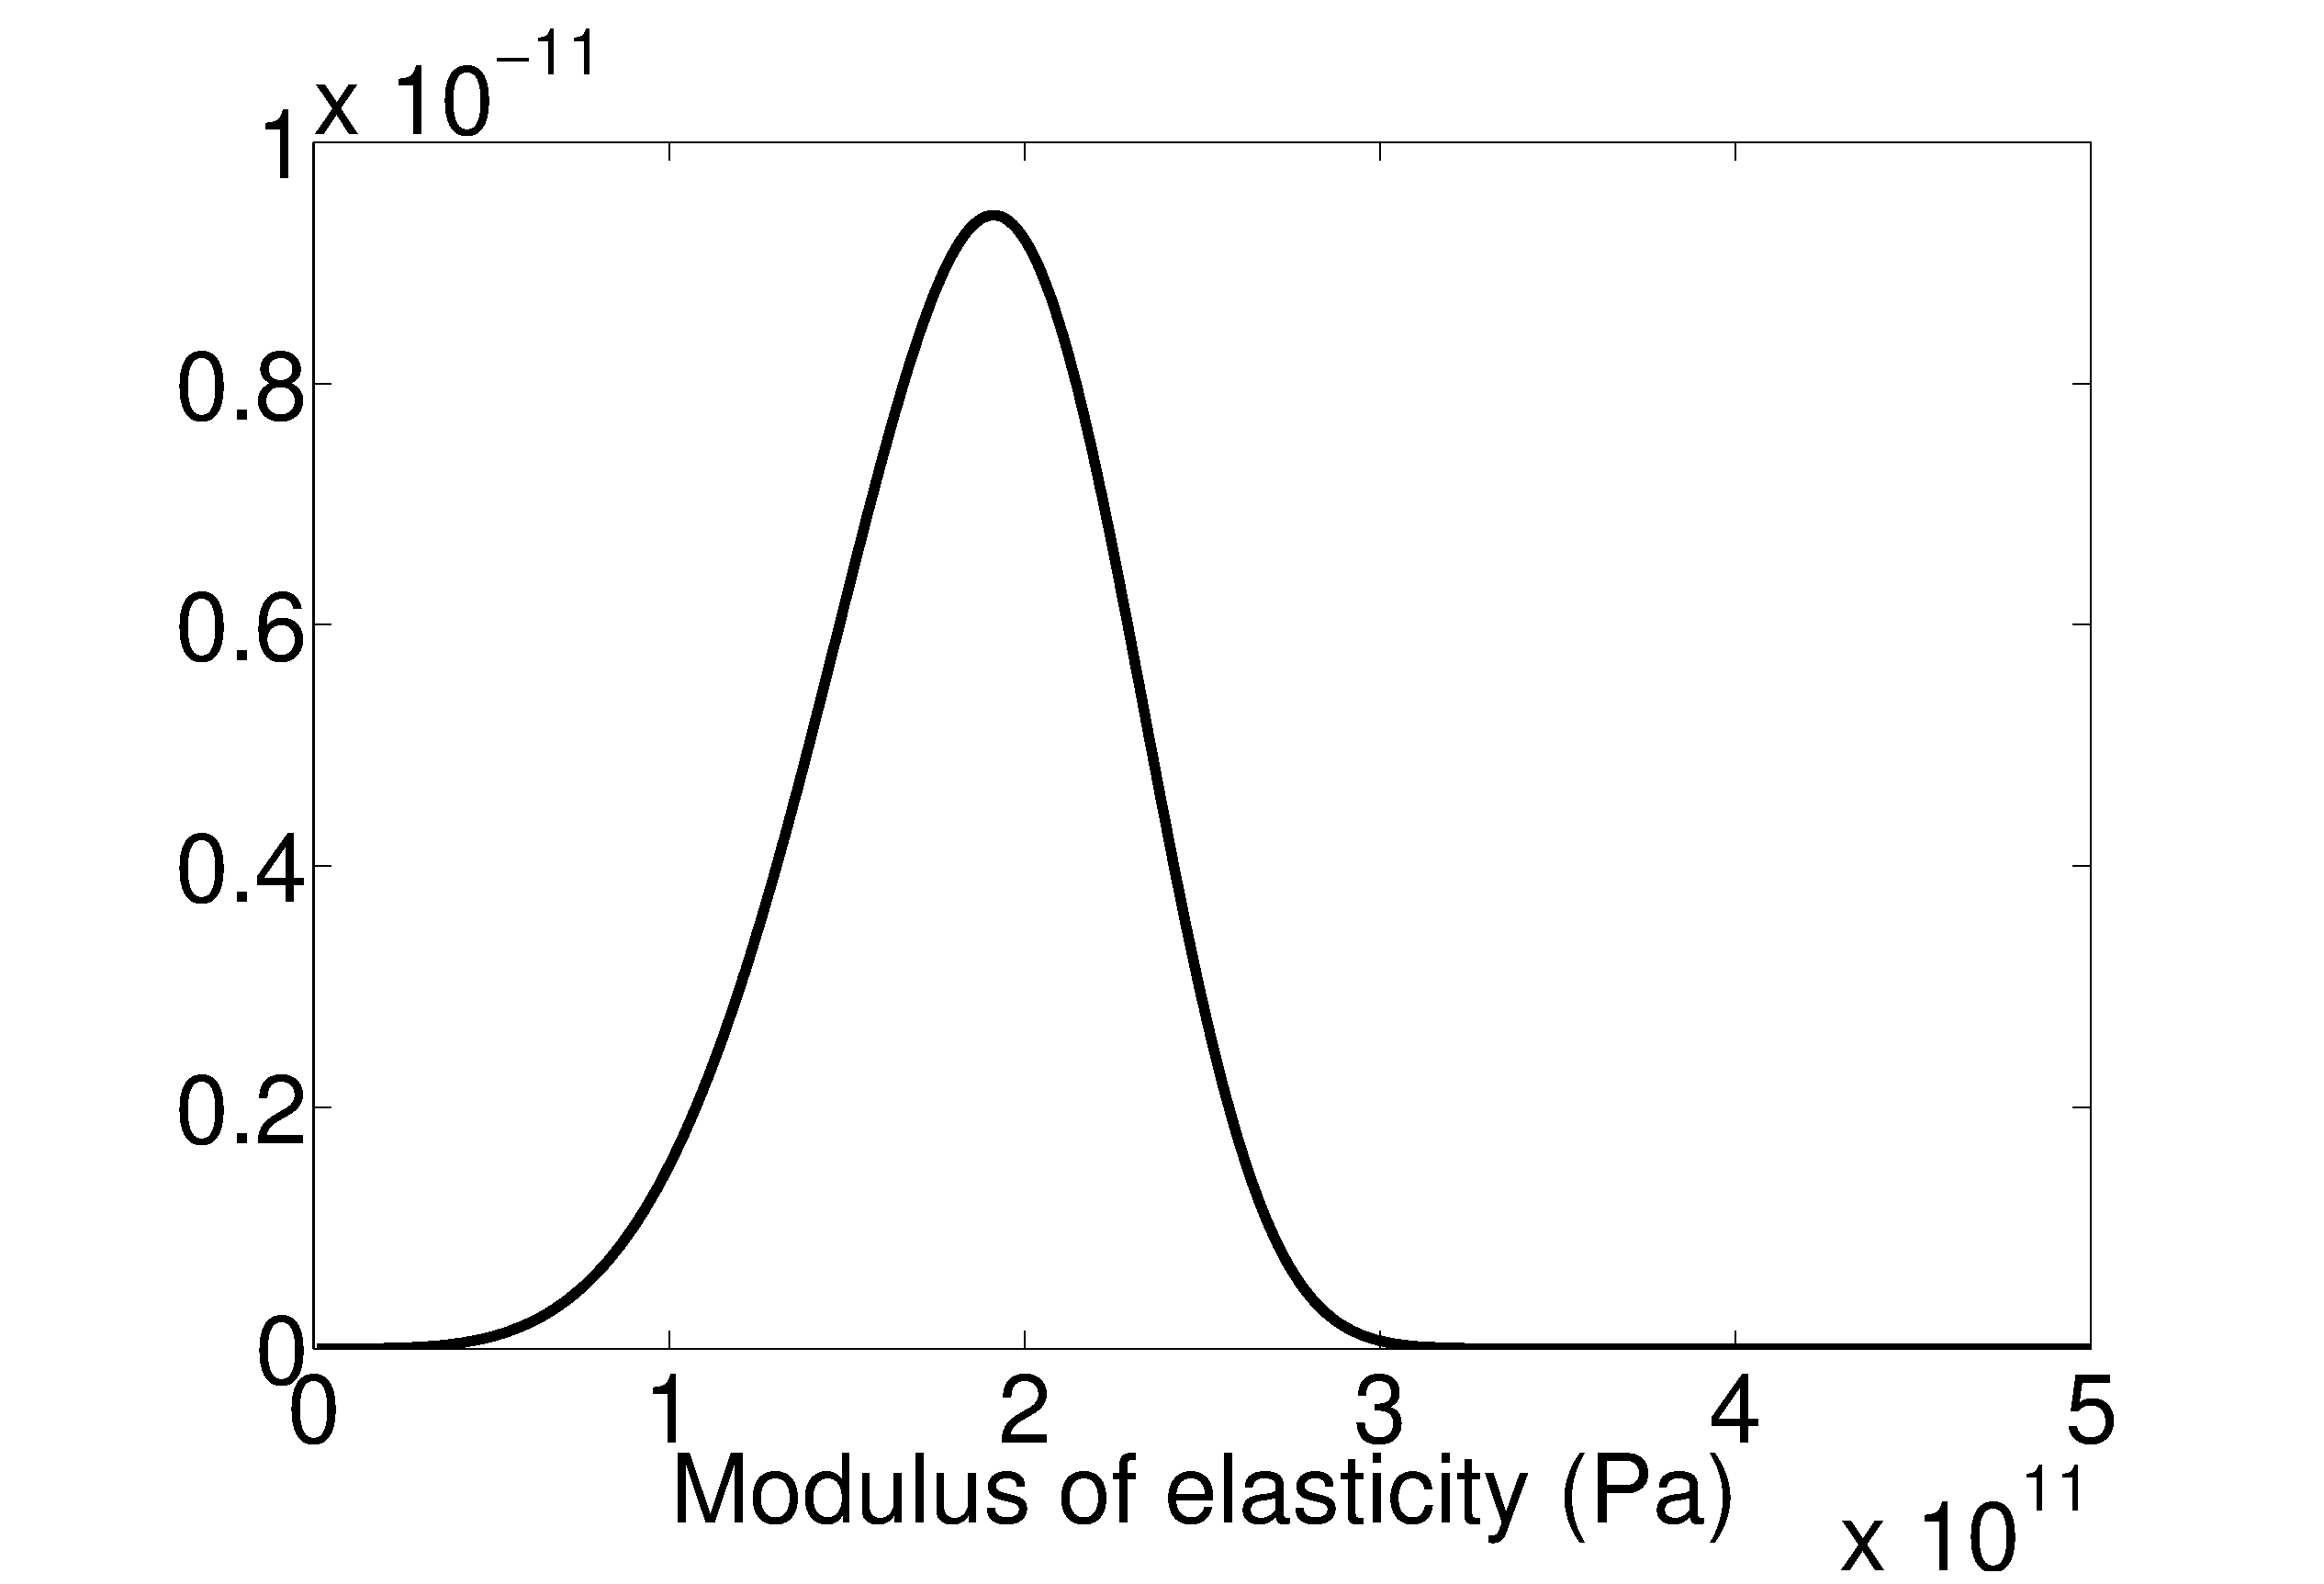
\includegraphics[height=5.15cm]{modulus_of_elasticity_pdf.eps}
		\label{fig:results_fft}
		}
		\quad
		\subfigure[Connection point location PDF.]
		{
		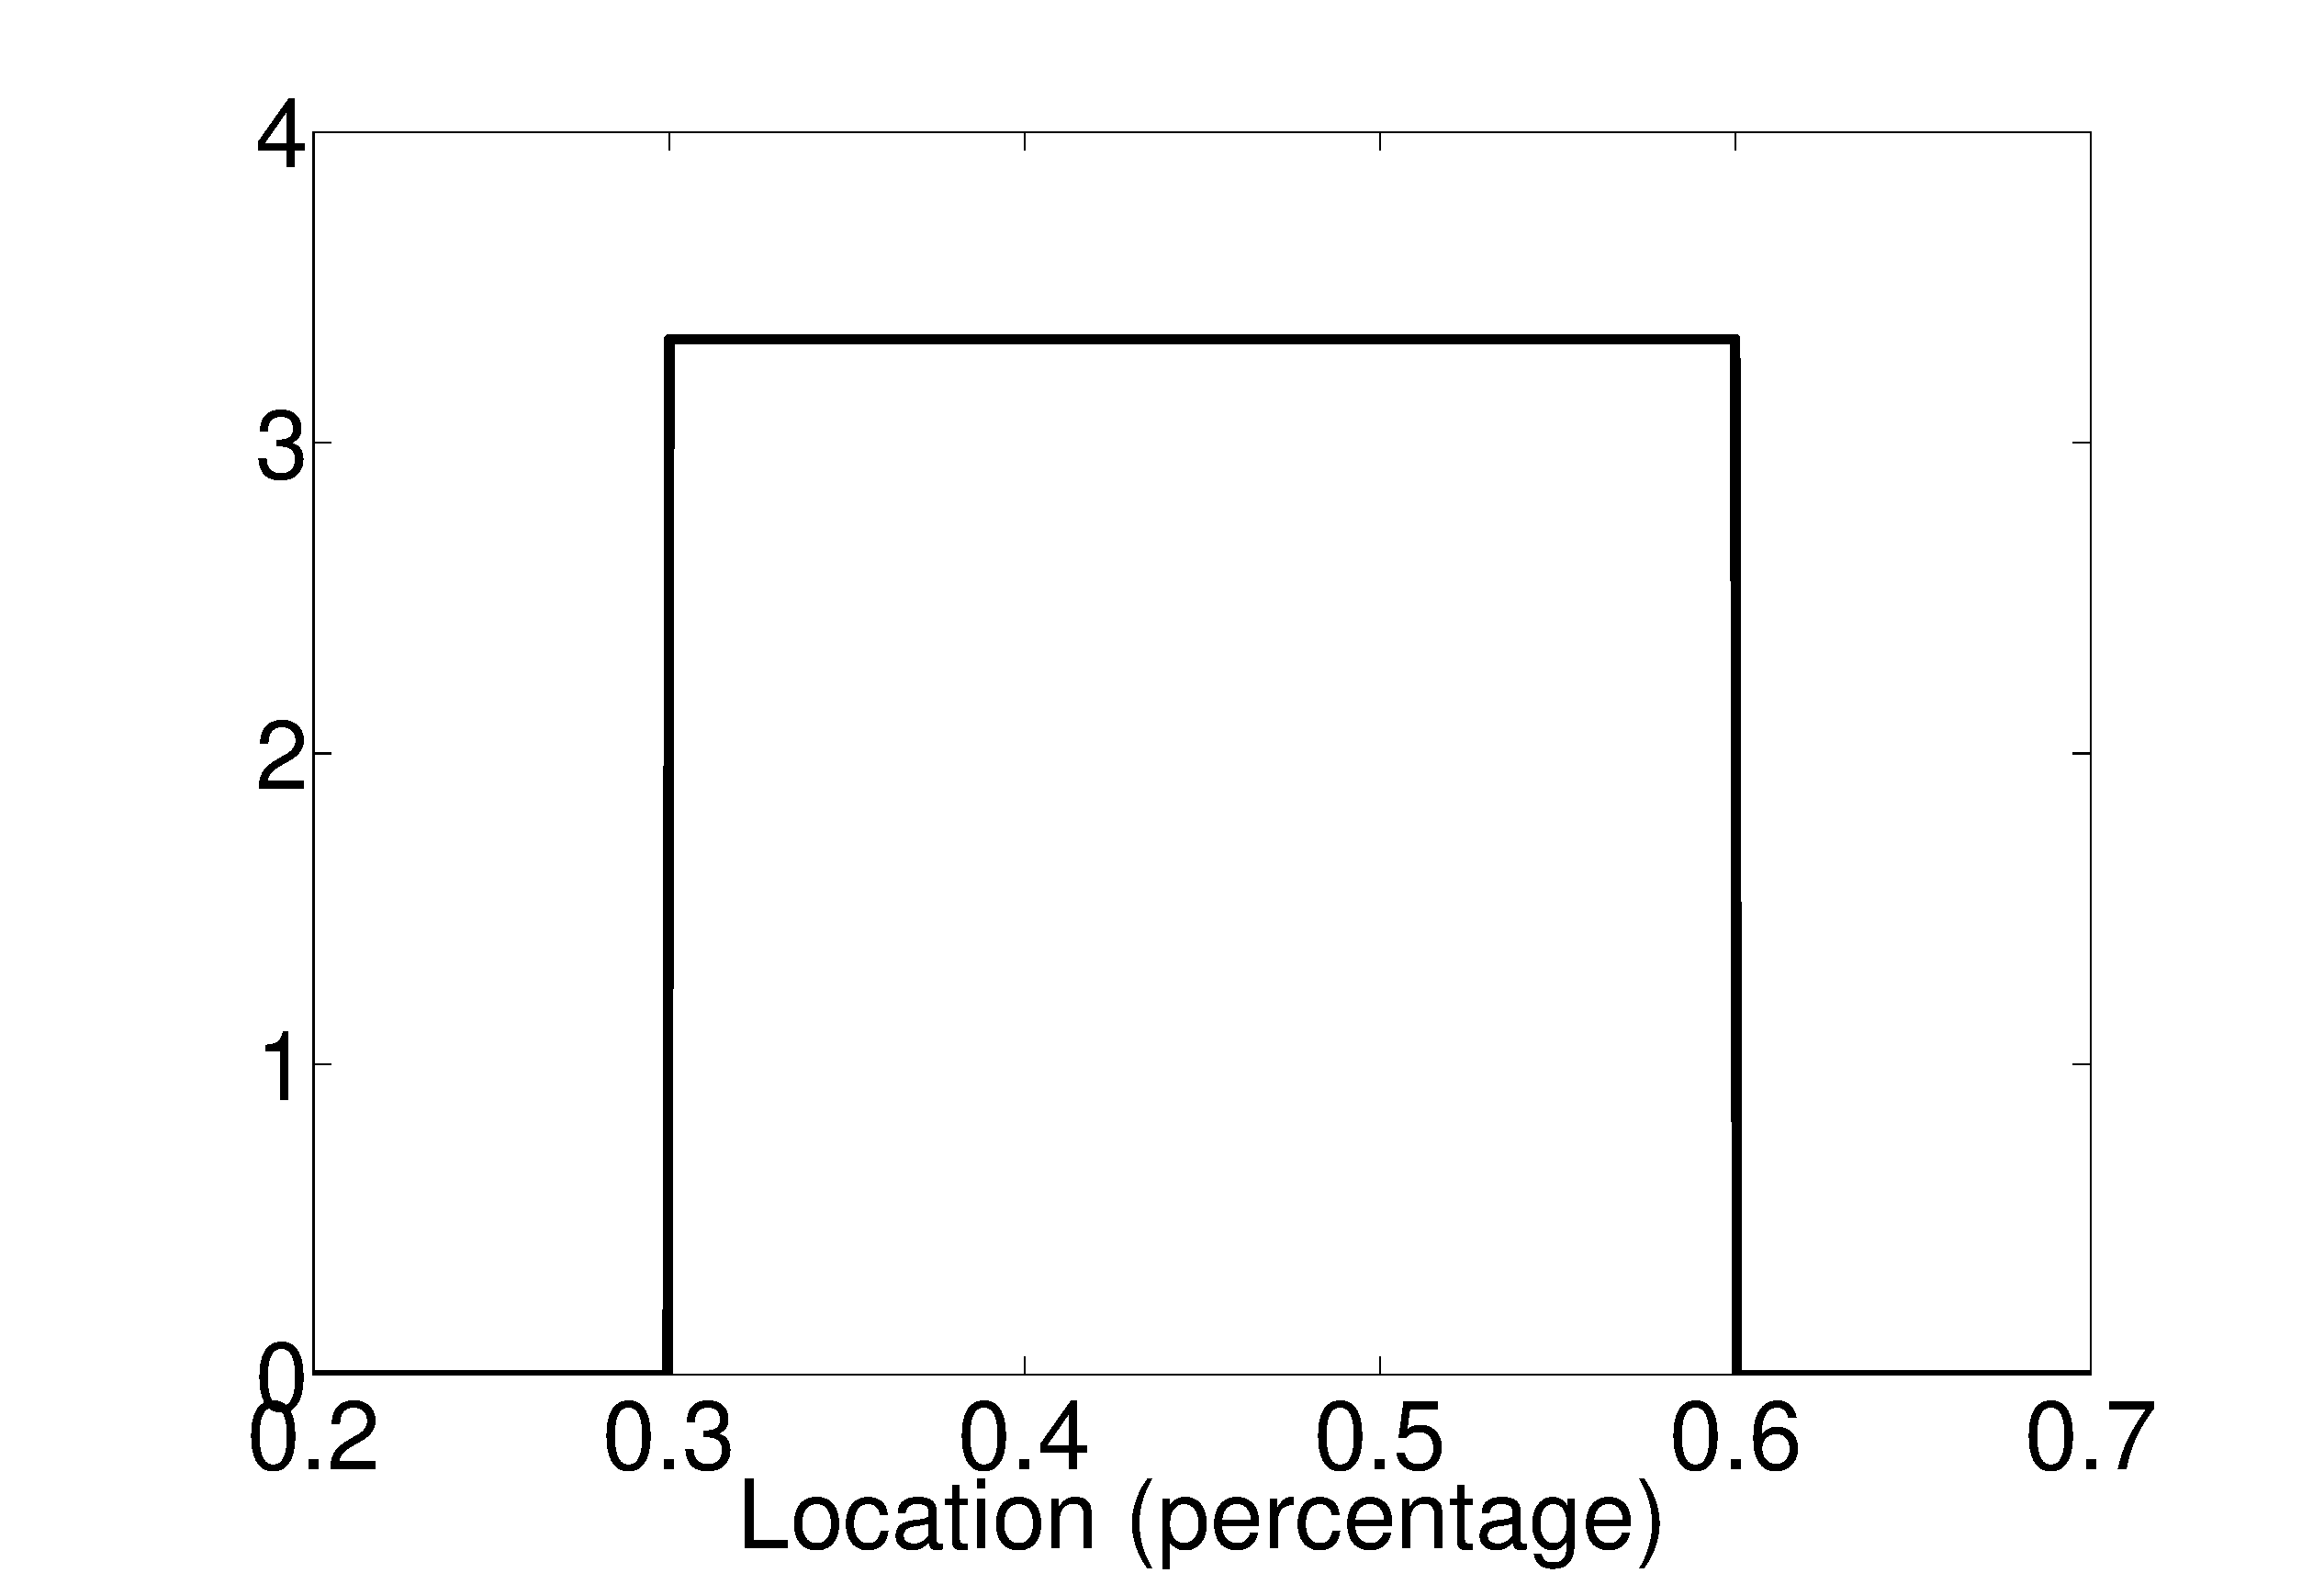
\includegraphics[height=5.15cm]{location_pdf.eps}
		\label{fig:results_hist}
		}
		\\
		\subfigure[Length of wing PDF.]
		{
		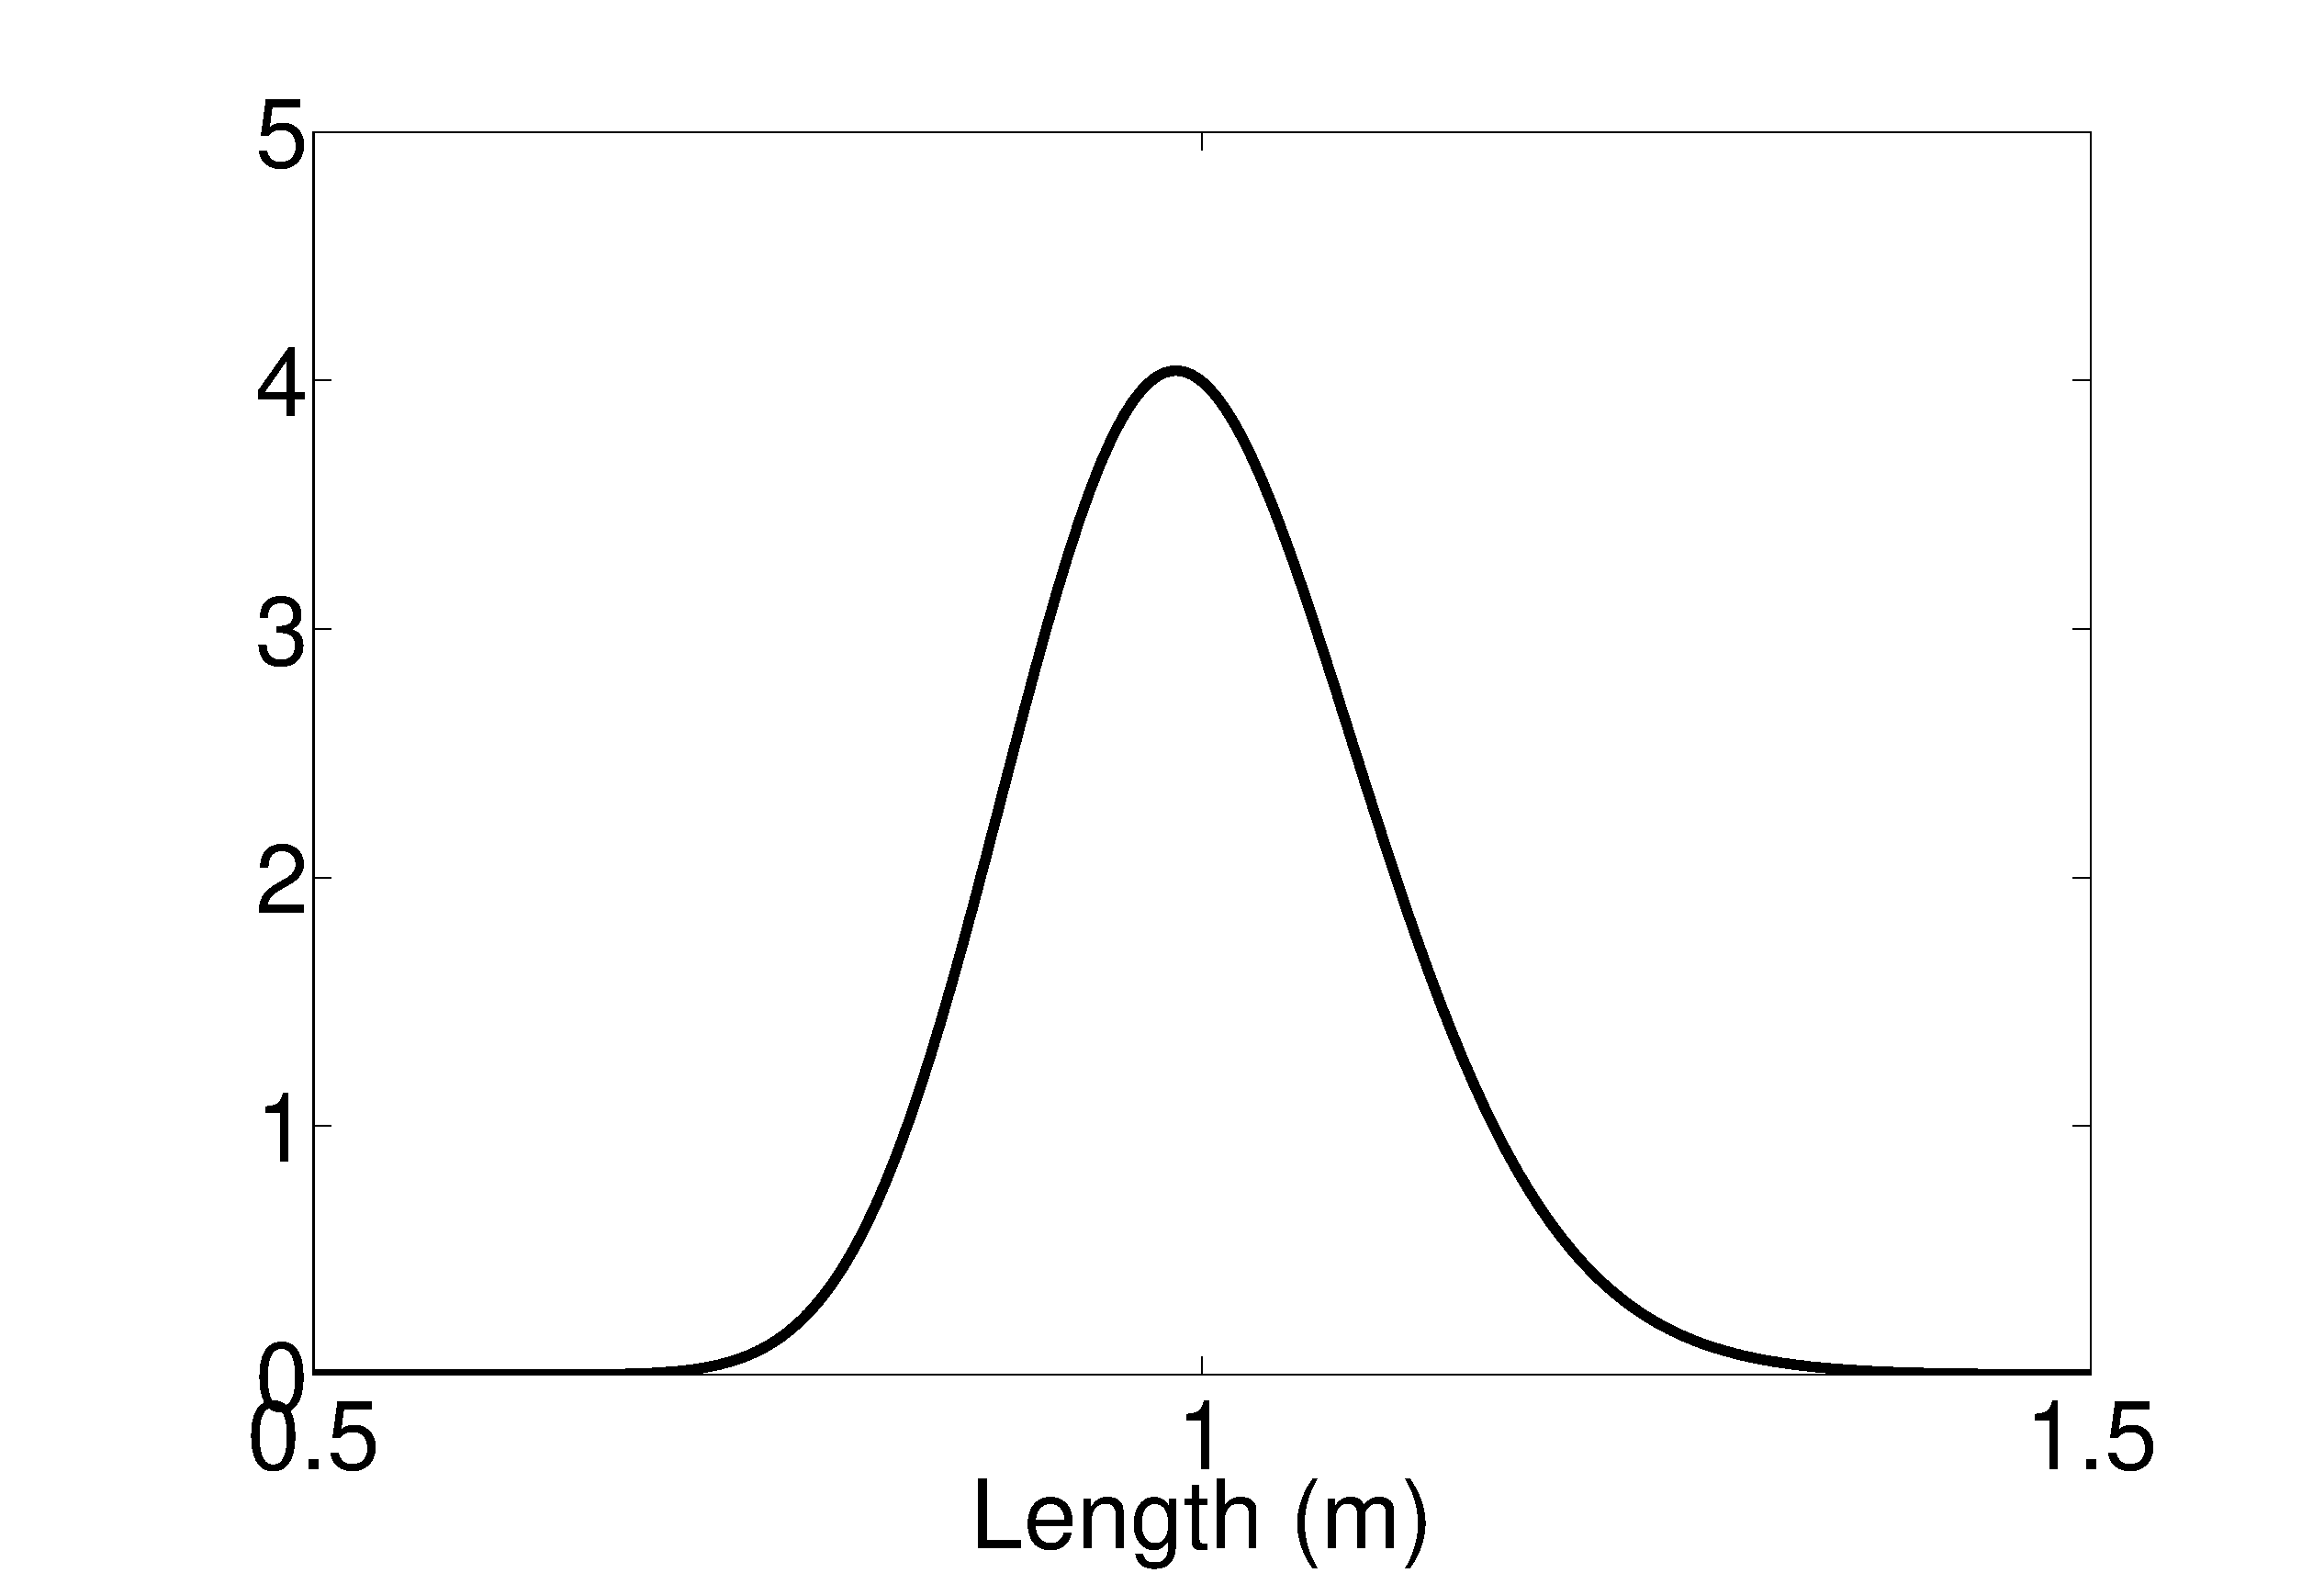
\includegraphics[height=5.15cm]{length_pdf.eps}
		\label{fig:results_fft}
		}
		\quad
		\subfigure[Area moment of inertia PDF.]
		{
		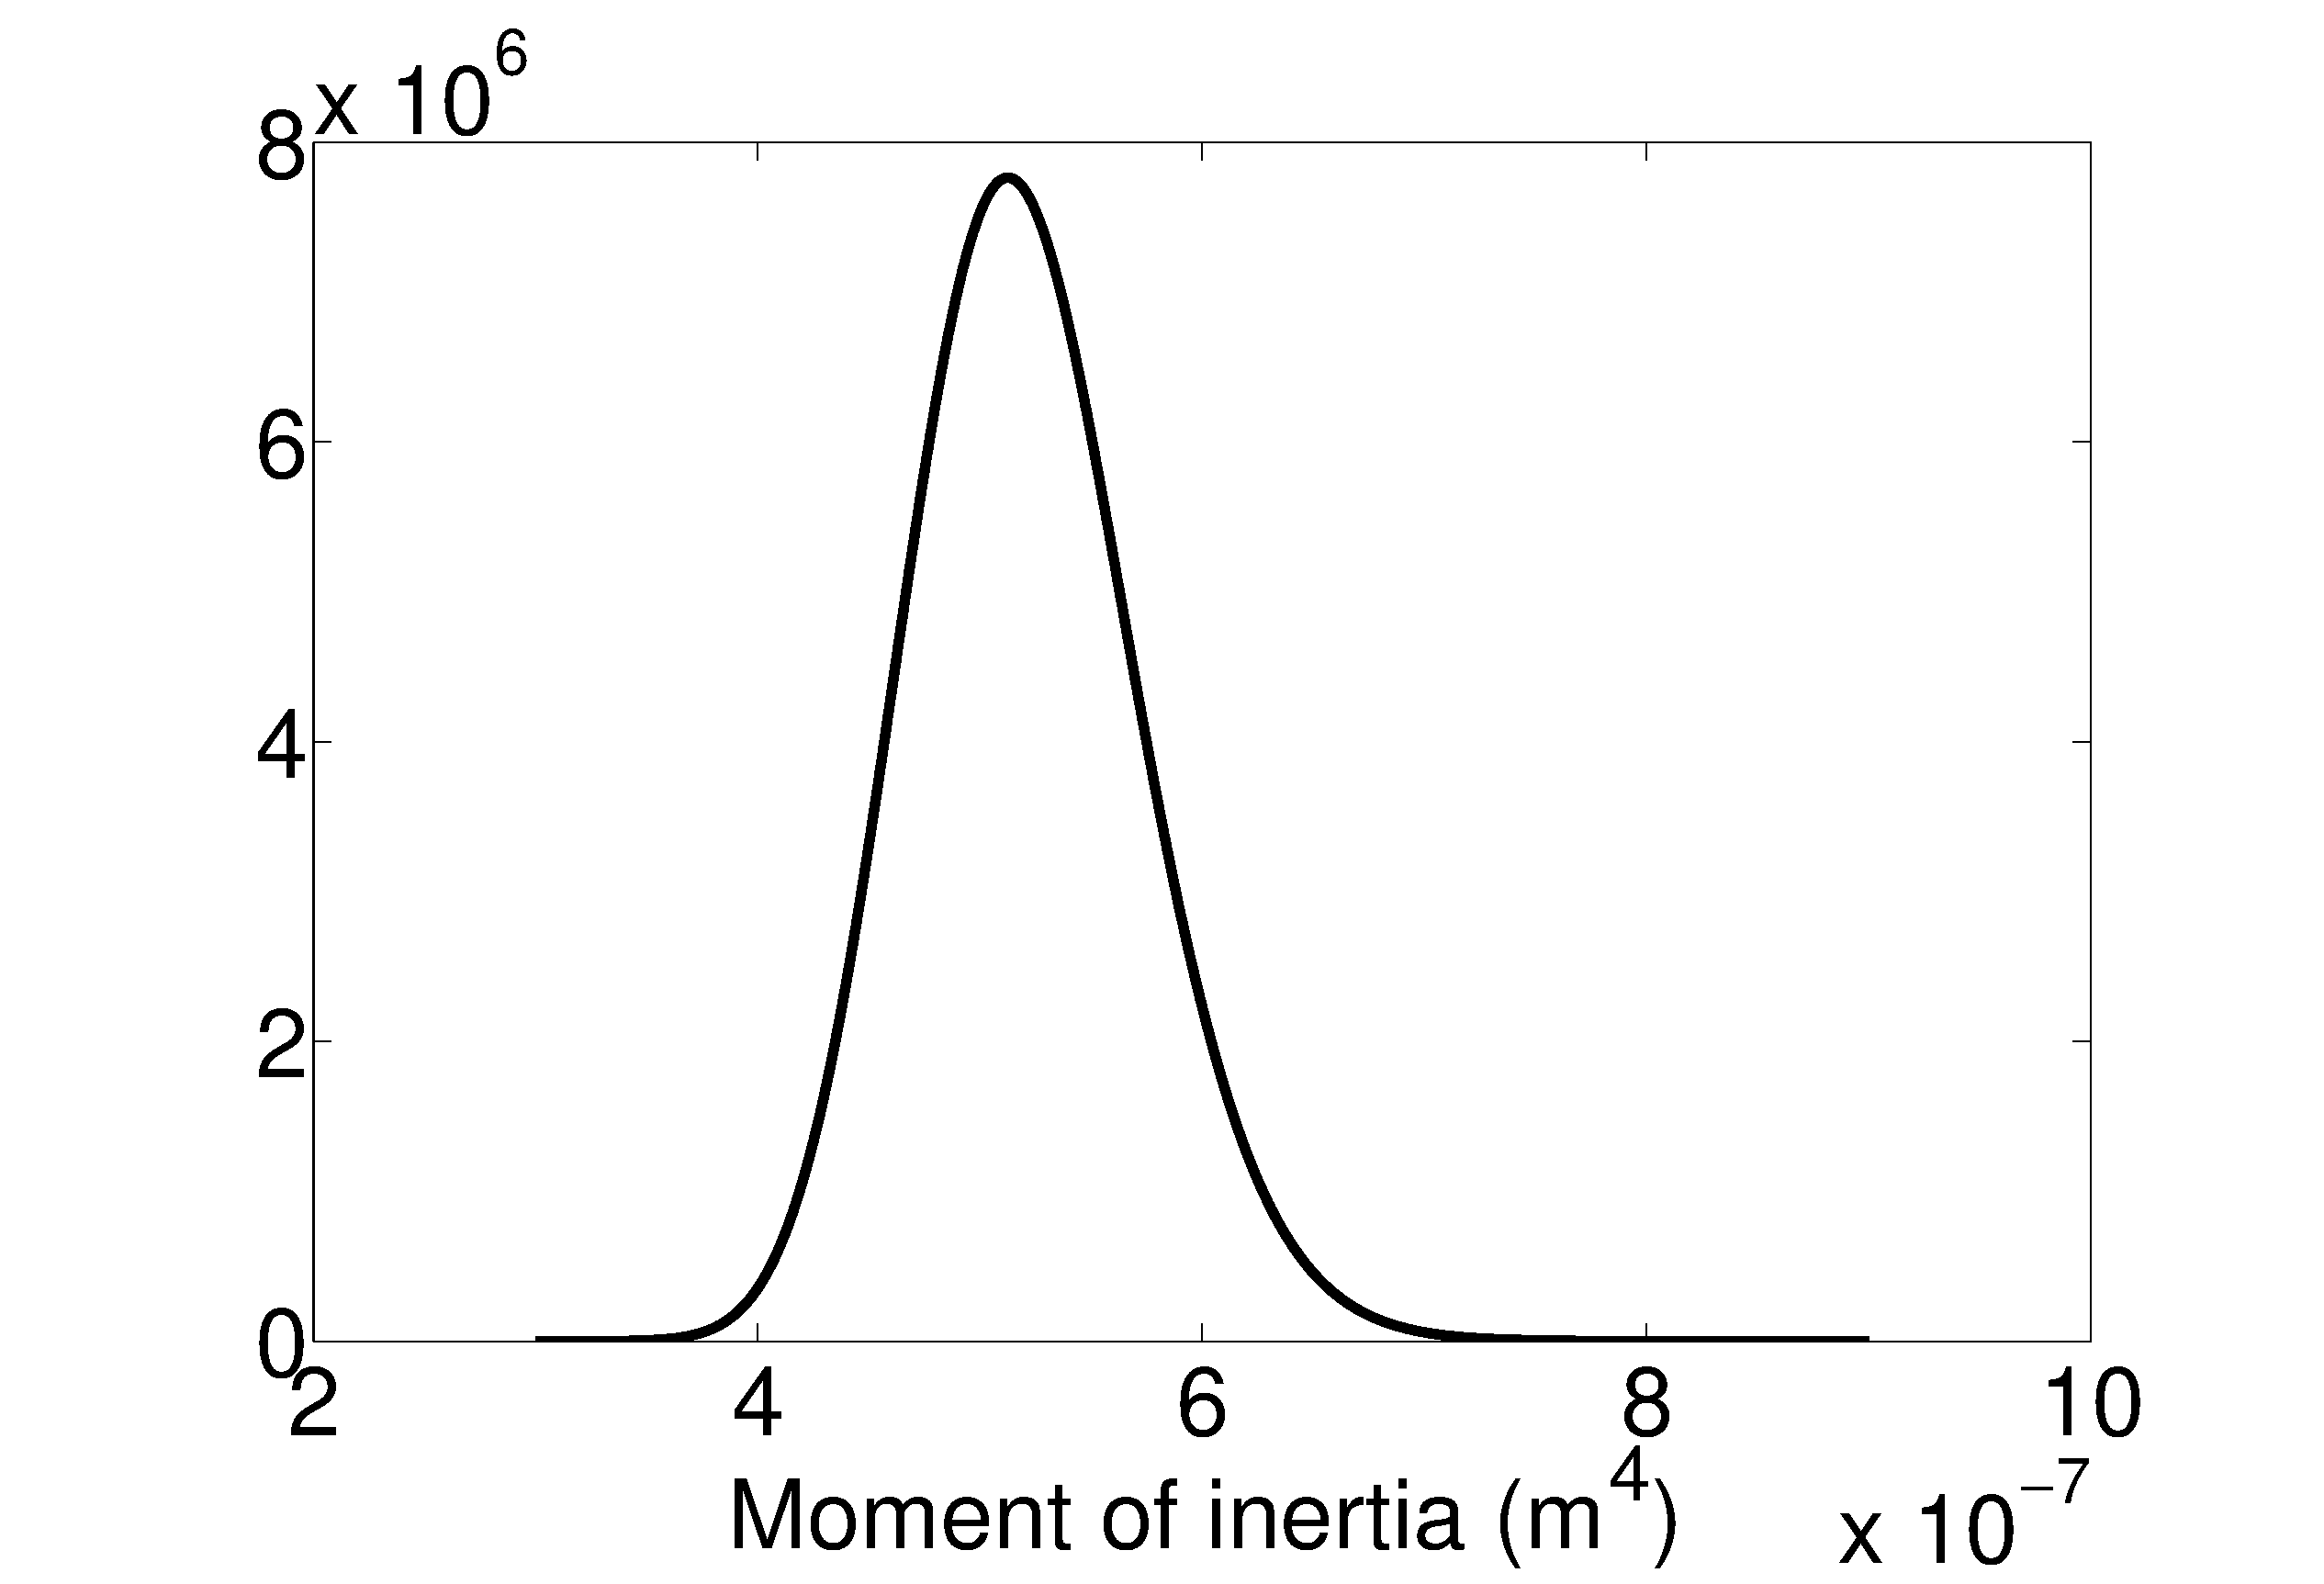
\includegraphics[height=5.15cm]{moment_of_inertia_pdf.eps}
		\label{fig:results_hist}
		}
		\caption{Random variables probability distribution function (PDF).}
		\label{fig:random_variables_pdf}
	\end{figure}
%
% --------------------------------------------------------------------------------
\subsection{Sensitivity Analysis}
Although many parameters can be defined as uncertain for this problem, not all of them contribute to change the limit-state function. The effect of uncertain variables on the limit-state can be investigated by looking at the sensitivity of the limit-state. The large magnitudes for a sensitivity shows a large contribution of the variables where the sensitivity of the function is calculated with respect to.\\

The sensitivity of an arbitrary function, $F(X)$, to its variables, $x_i$, is defined as the derivative of the function with respect to that specific variable. Since there are no closed form equation available for the limit-state of this problem, the derivatives are numerically calculated as shown in Equation \eqref{eq:sensitivity_FD}.
%
\begin{gather}\label{eq:sensitivity_FD}
	\frac{dF(x_1,x_2,\dots,x_n)}{dx_i} = \frac{F(x_1,x_2,\dots,x_i + dx_i,\dots,x_n) - F(x_1,x_2,\dots,x_i,\dots,x_n)}{dx_i}
\end{gather}
%
The crucial concern when using the finite difference approach is selection of the step size. Step size has a big effect on the sensitivity results. Therefore, it is needed to study the convergence of step-size and choose the most accurate one. The sensitivity and convergence history of the different random variables for this problem is shown in Figure ~\ref{fig:sensitivity_FD_stepsize}. As shown in Figure ~\ref{fig:sensitivity_FD_stepsize} the step size of $1$ percent change in the original variable will provide a converged solution in finite difference results for almost all the variables. For the wind angle this changed to $0.5$ percent. Moreover, as shown in Figure ~\ref{fig:sensitivity_FD_stepsize} it can be concluded that decreasing the step does not necessary results in increase in the accuracy of the finite difference. The reason is because a small change in the numerator, which is small change in limit-state due to small change in design variable, is divided by a small value. This causes the sensitivities to be inaccurate for really small step sizes (truncation error). Another observation from Figure ~\ref{fig:sensitivity_FD_stepsize} is how much the different variables contribute to the change in the limit-state function. Finally, It should be noted that all these cases are done at the mean value of the distributions.
%
	\begin{figure}[H]
		\centering
		\subfigure[Sensitivity with respect to change in velocity.]
		{
		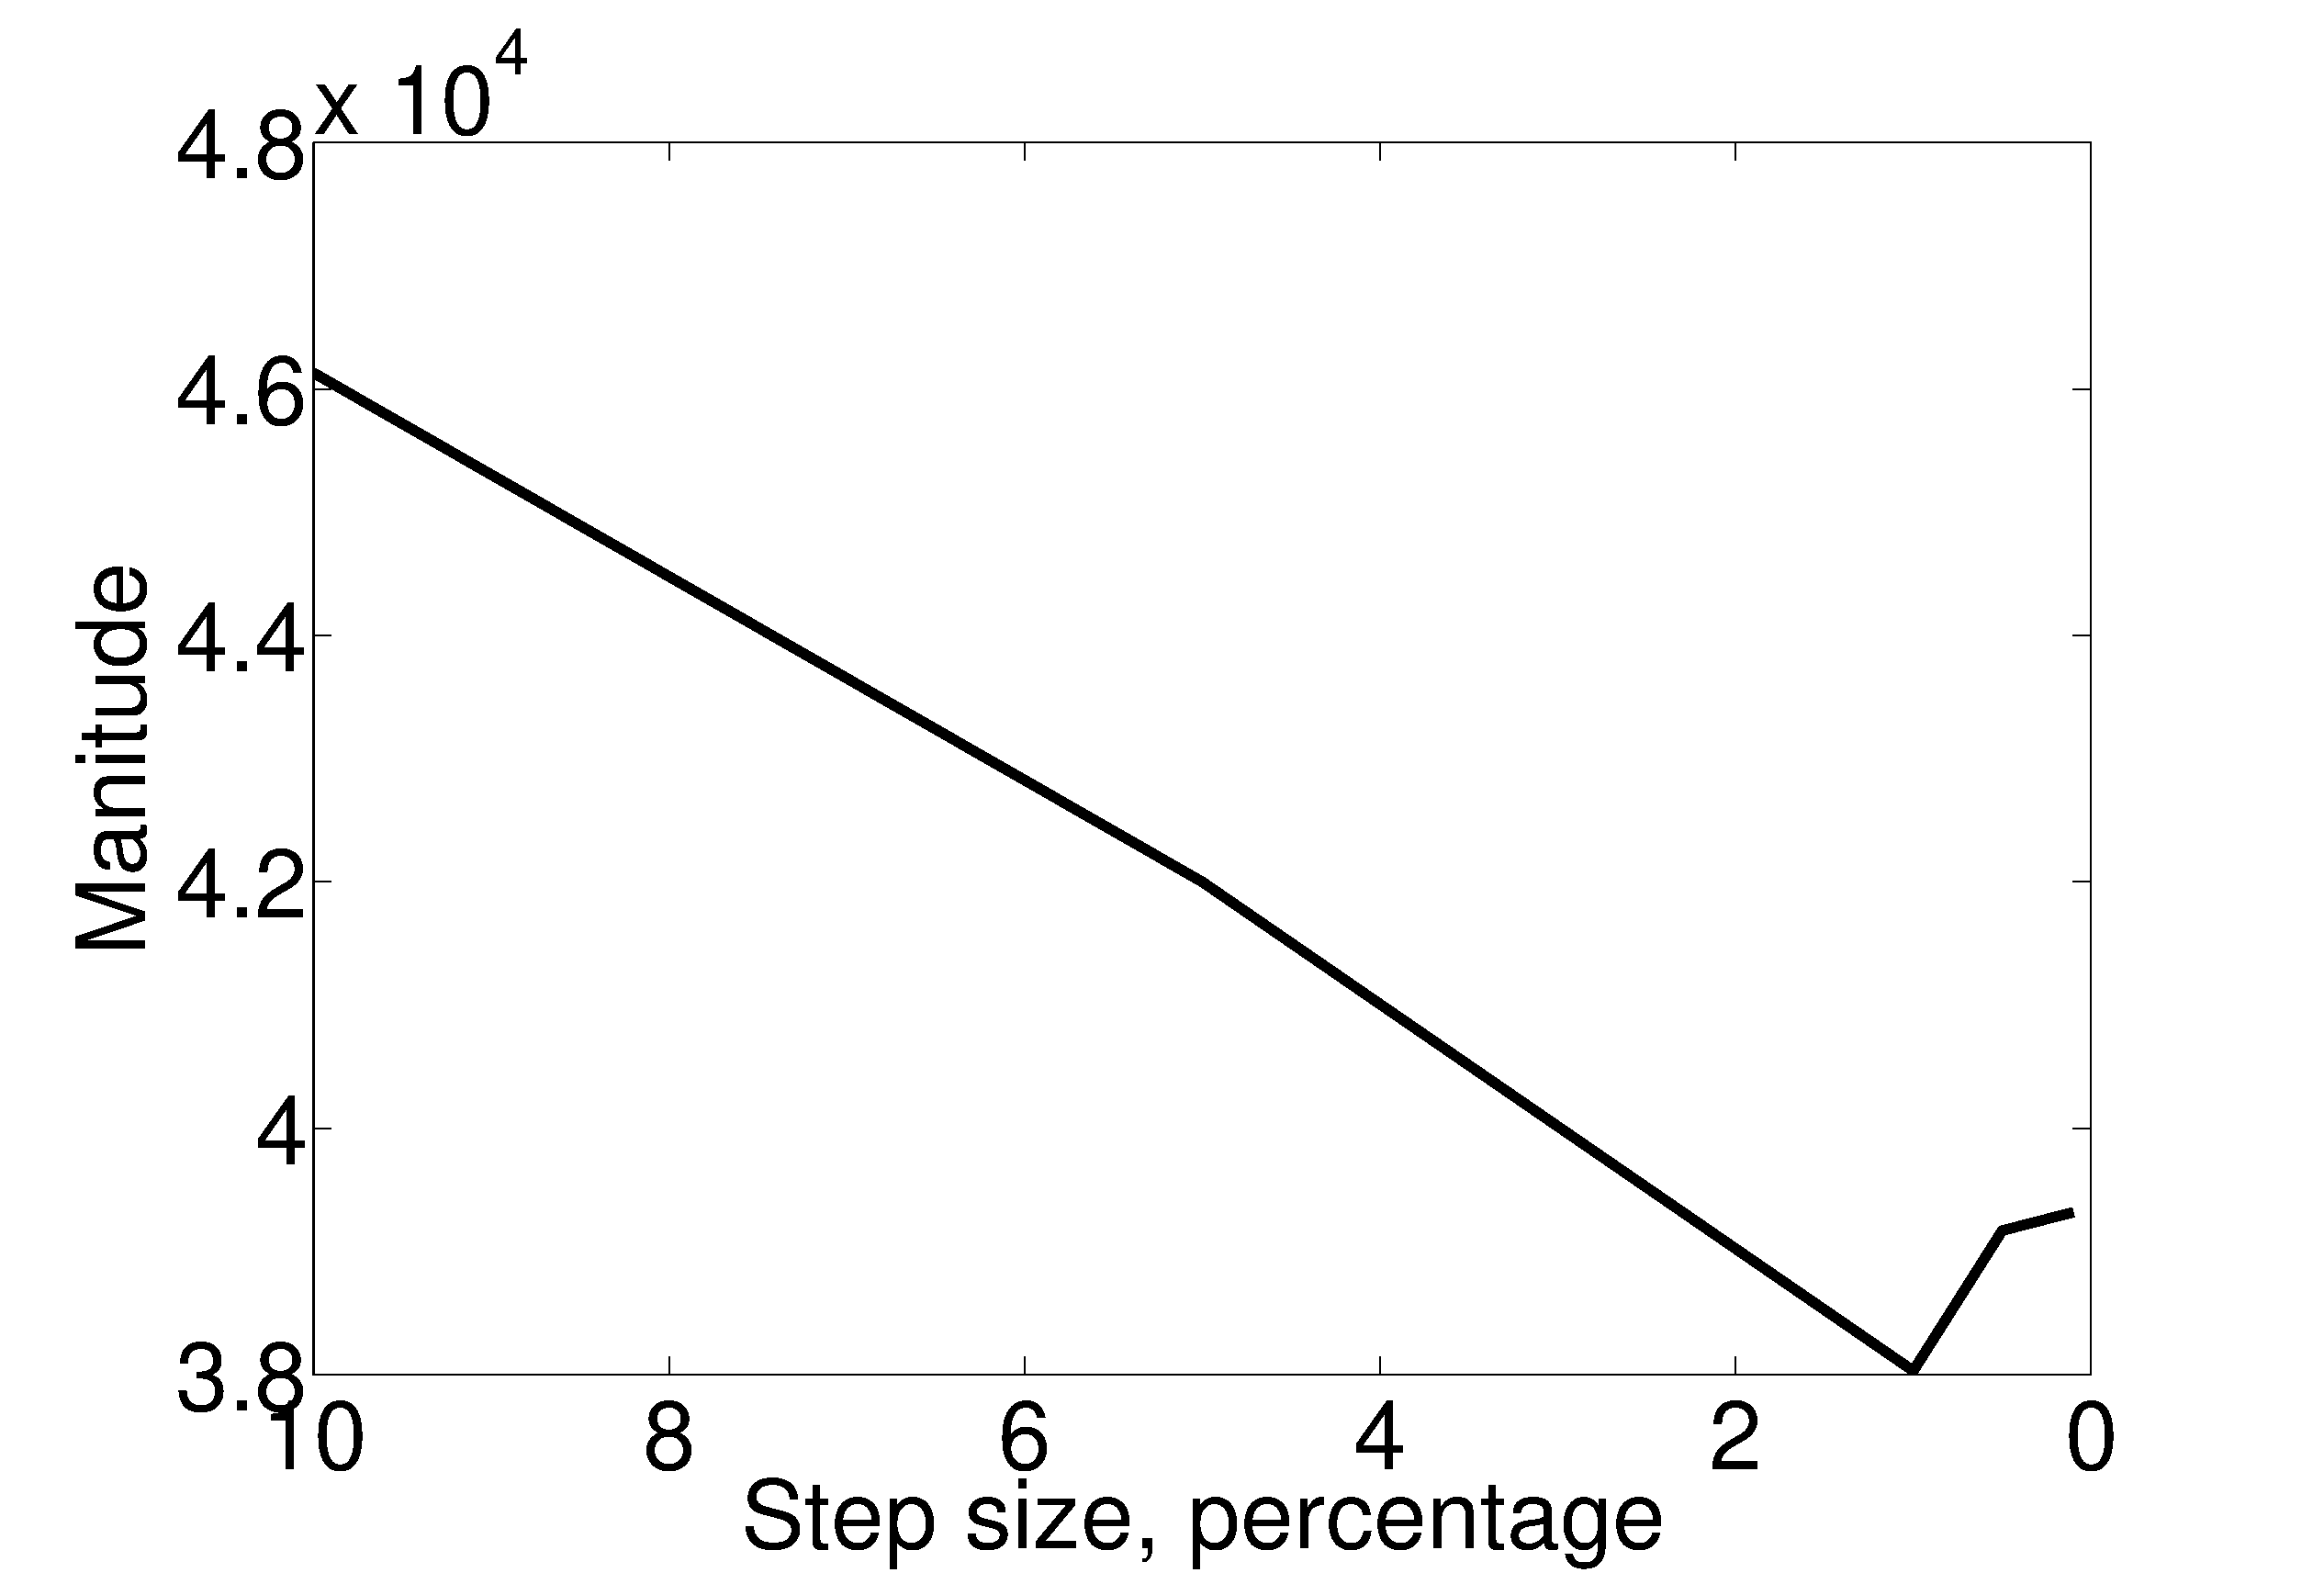
\includegraphics[height=5.15cm]{step_size_1.eps}
		\label{fig:results_fft}
		}
		\quad
		\subfigure[Sensitivity with respect to change in wind angle.]
		{
		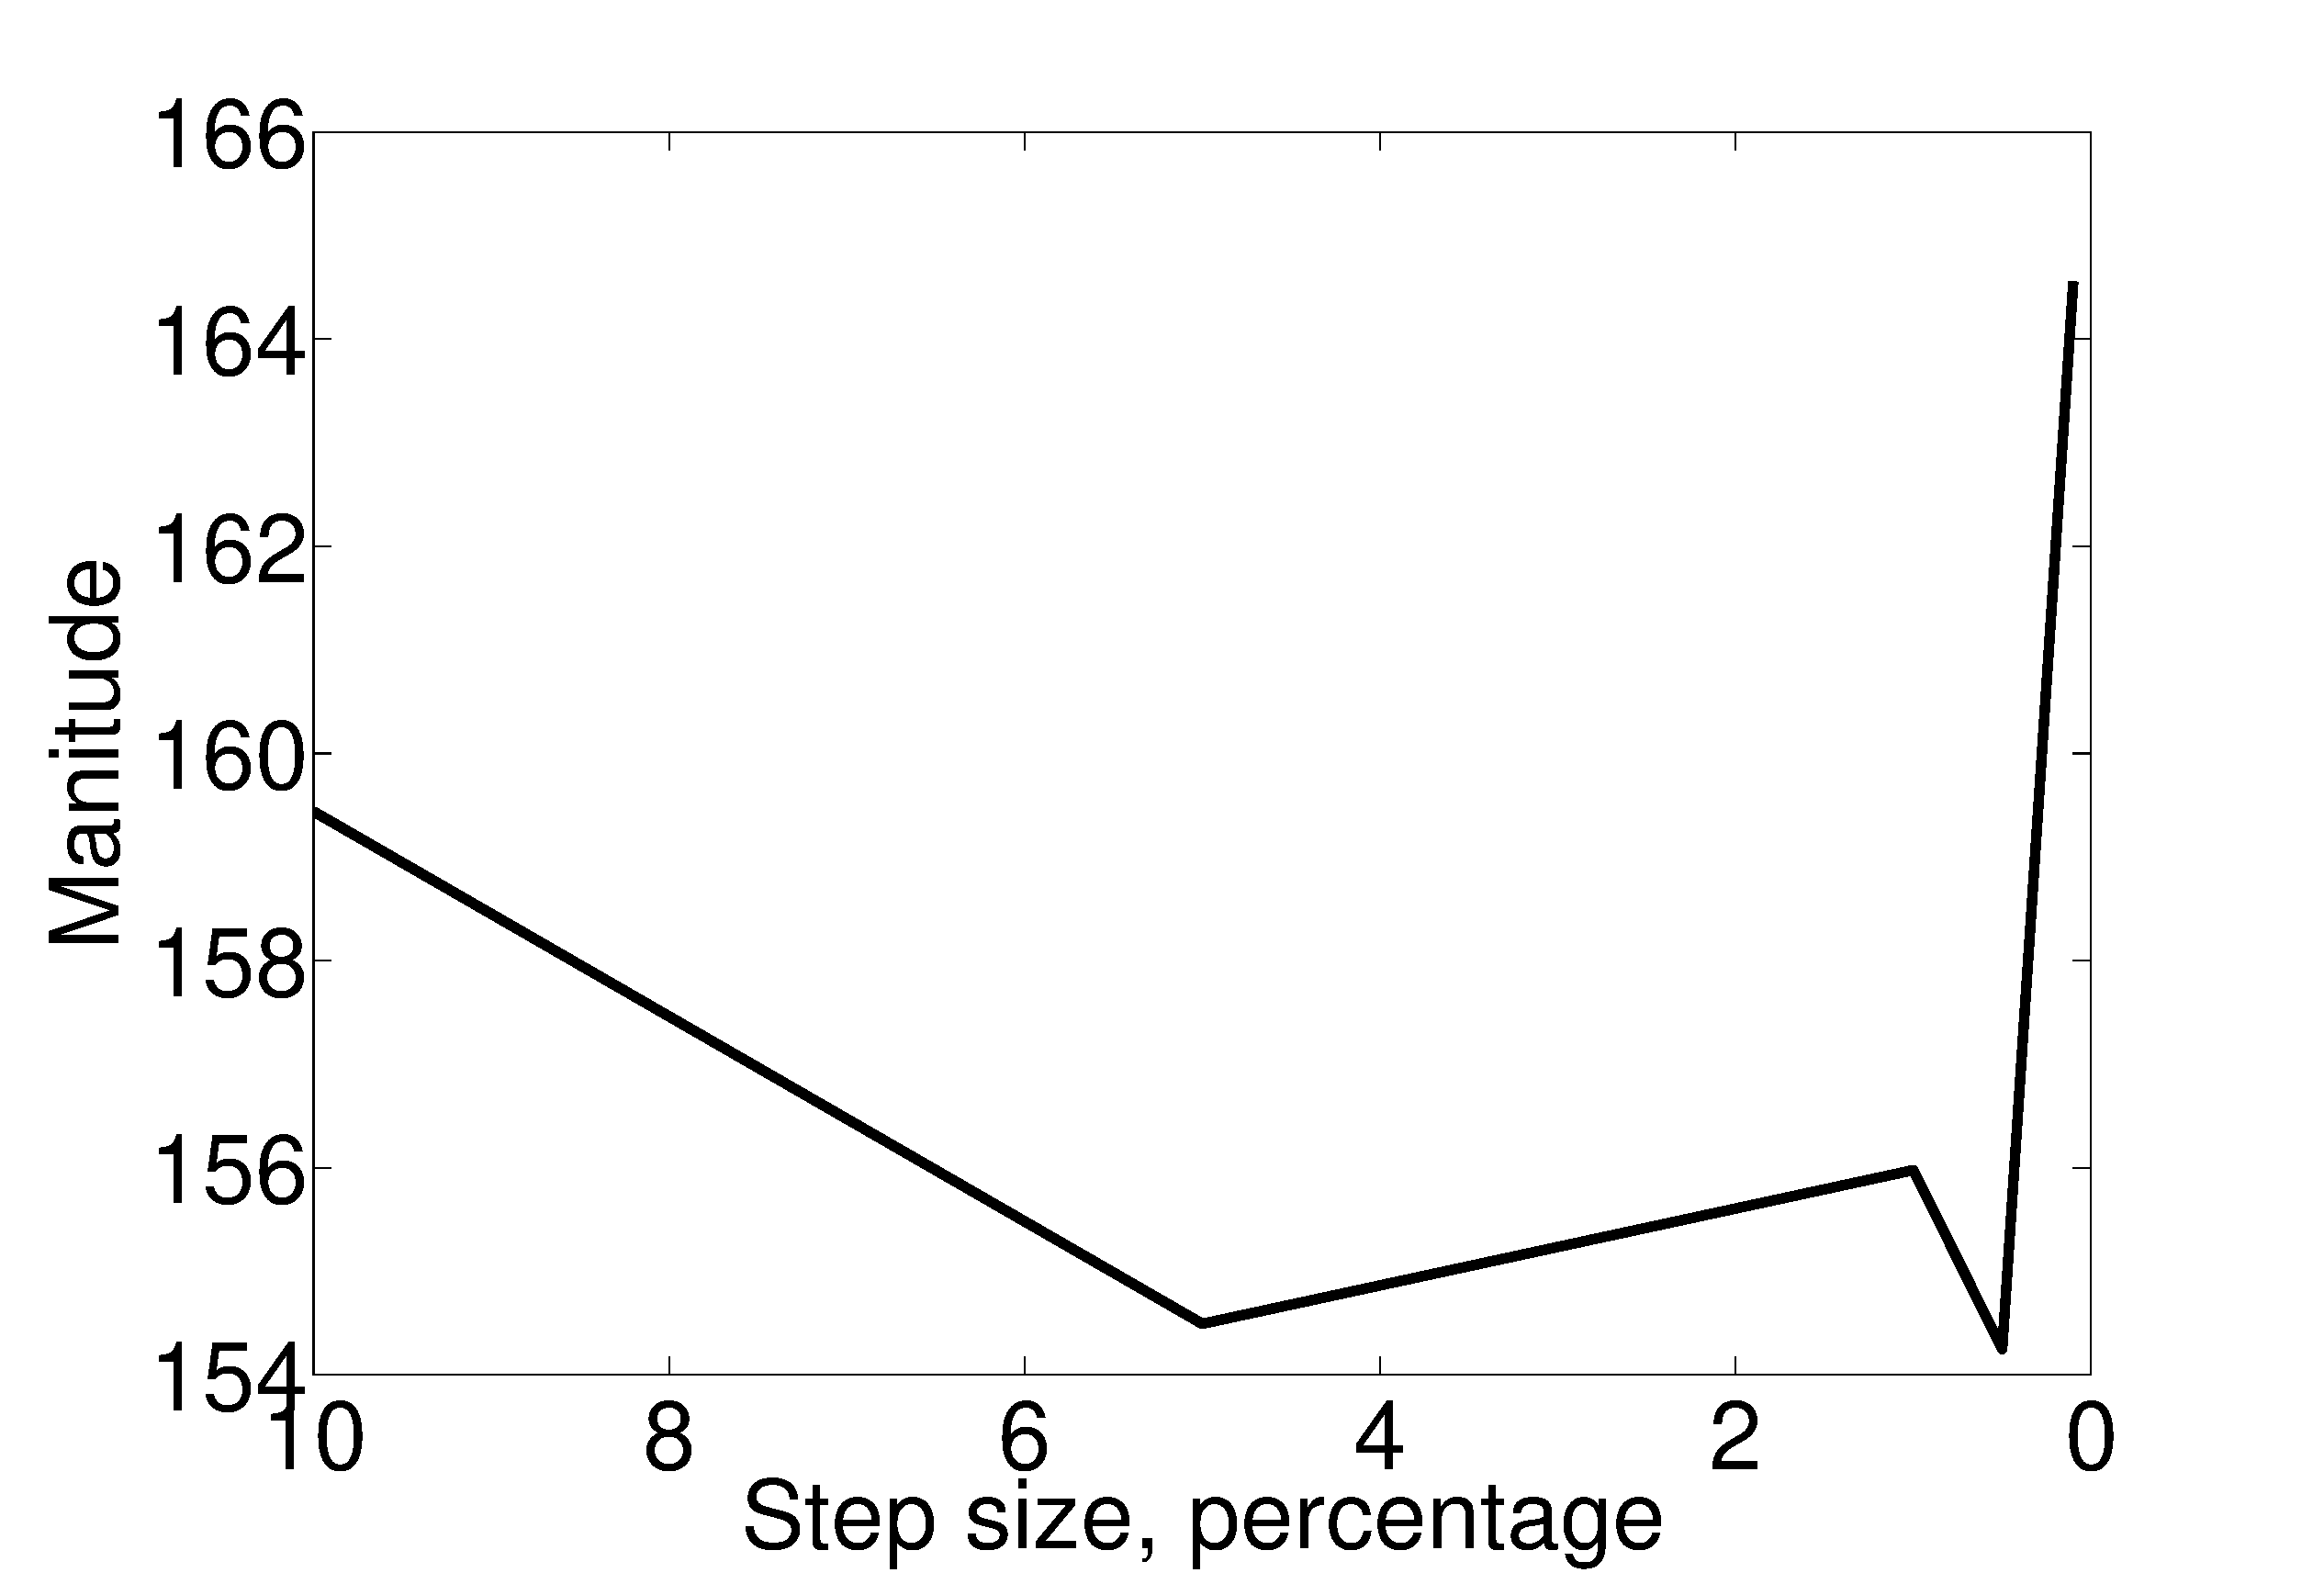
\includegraphics[height=5.15cm]{step_size_2.eps}
		\label{fig:results_hist}
		}
		\\
		\subfigure[Sensitivity with respect to change in connection point location.]
		{
		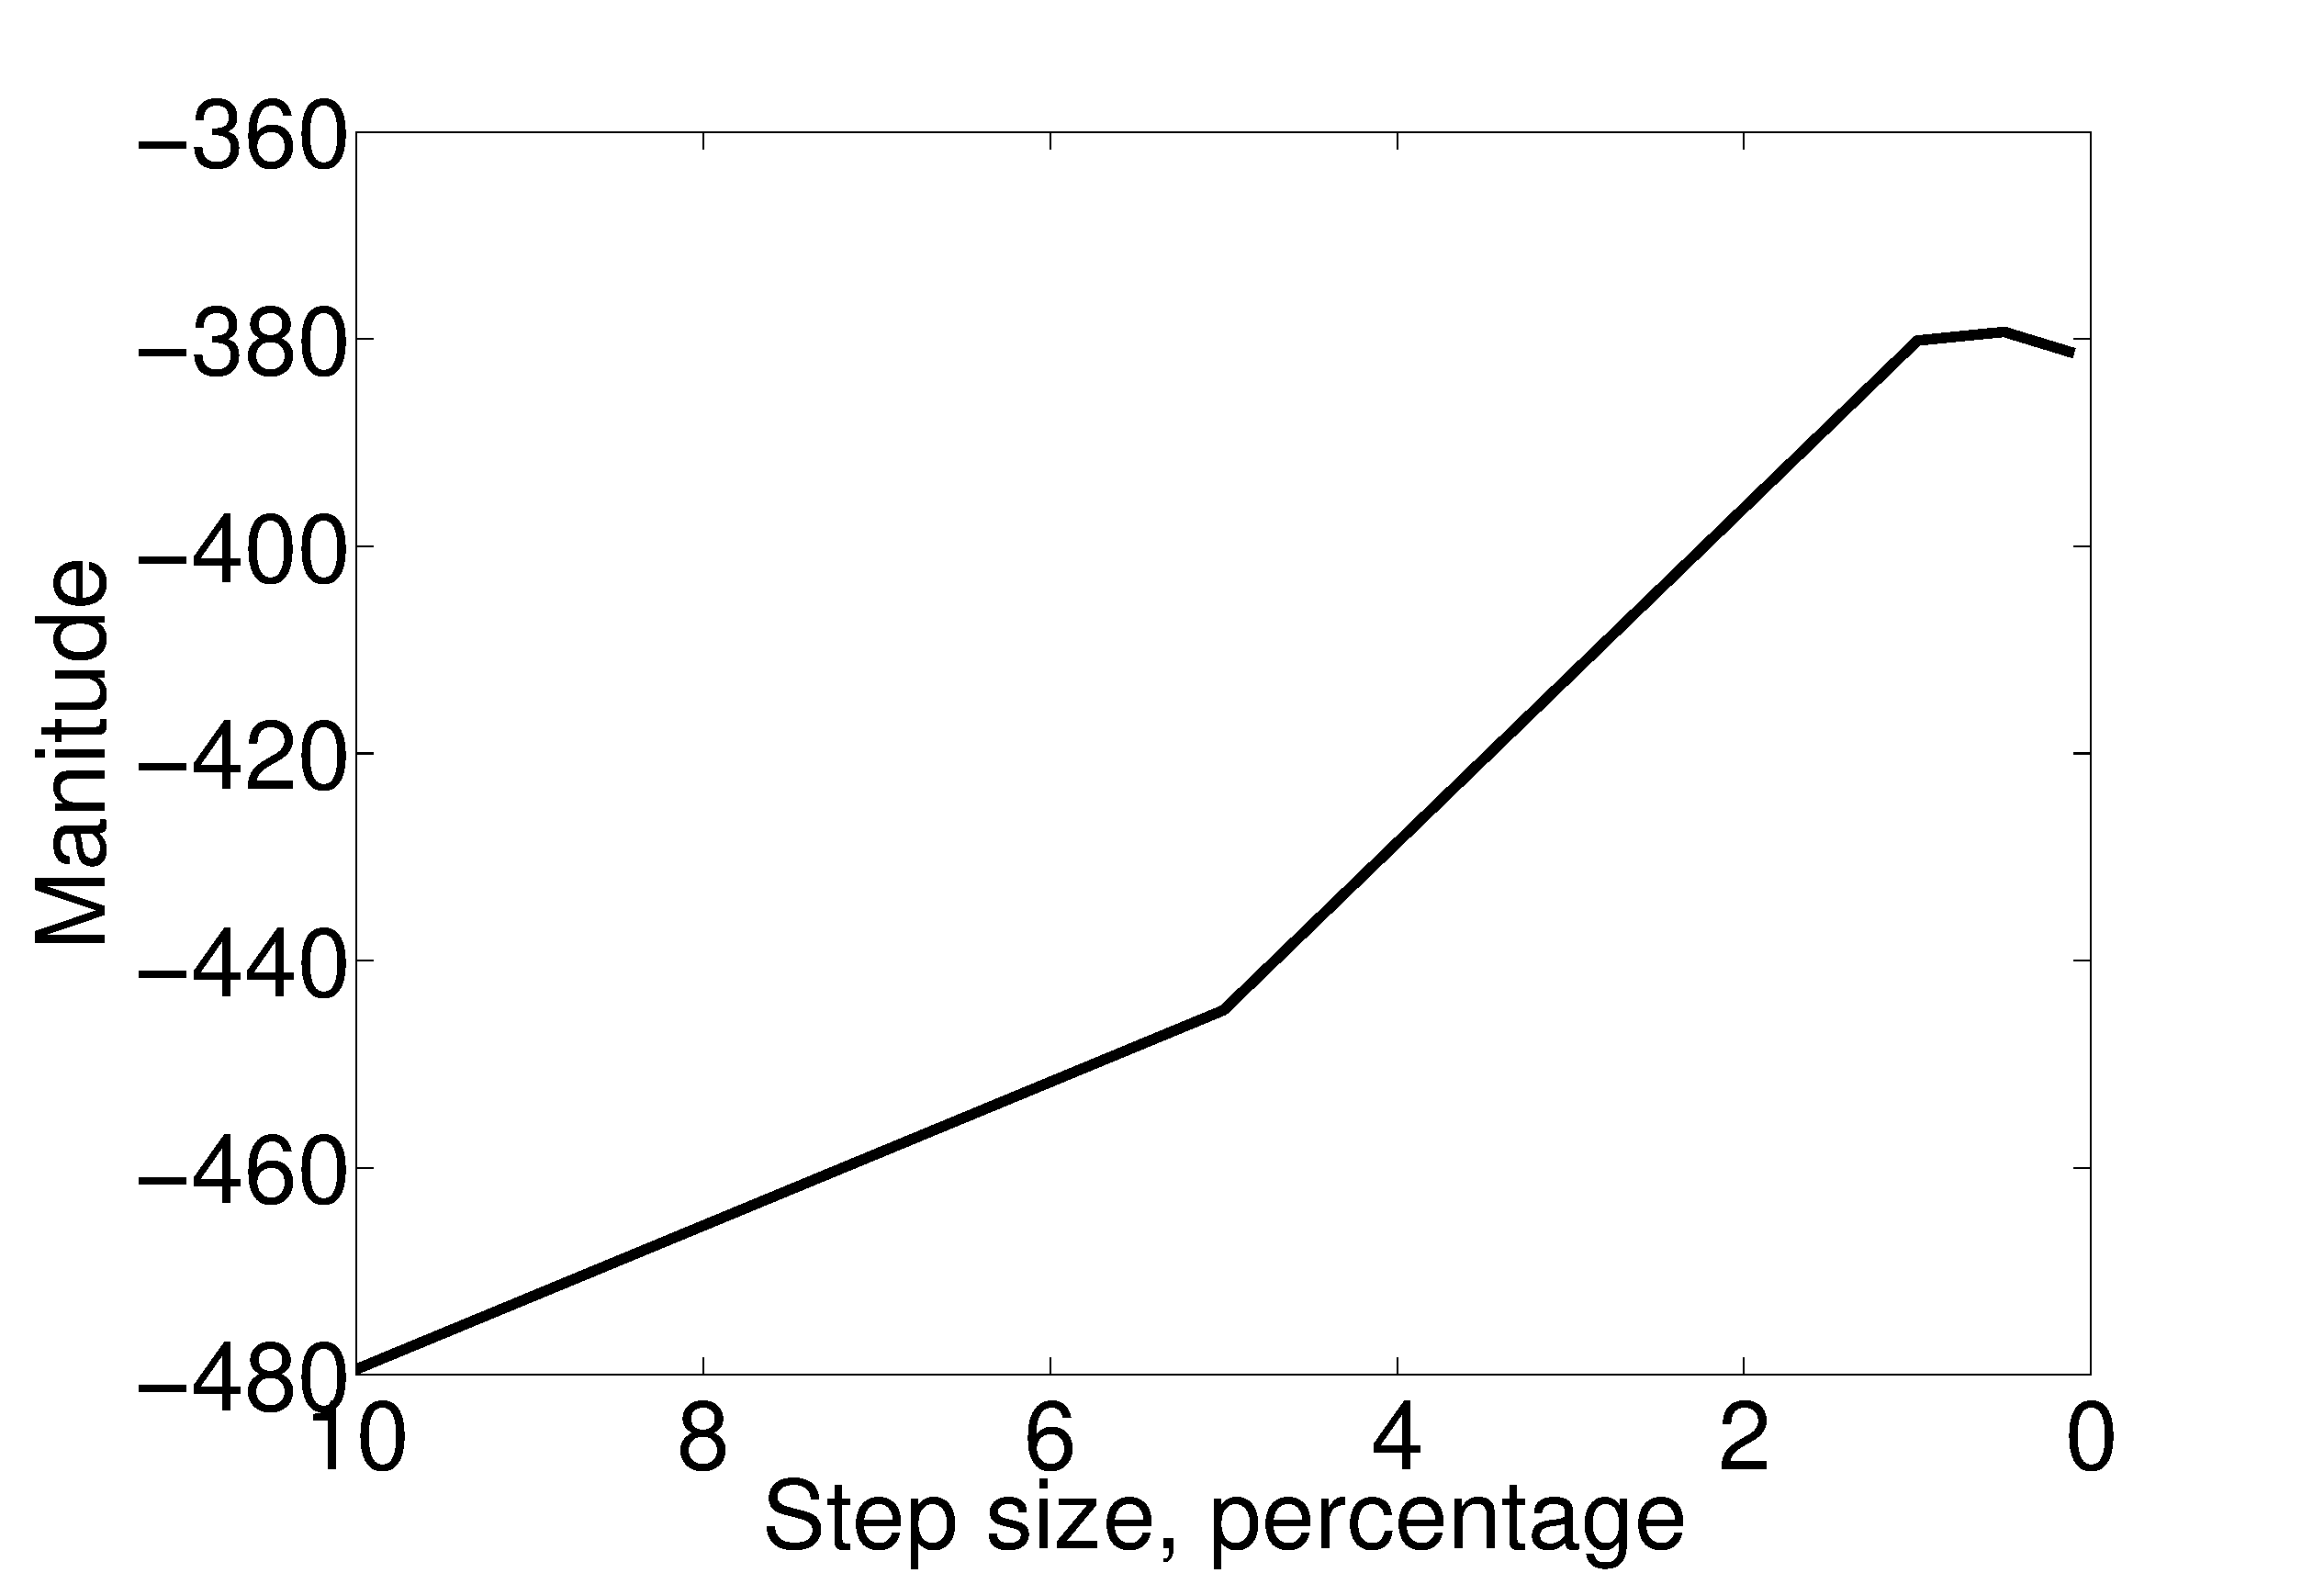
\includegraphics[height=5.15cm]{step_size_3.eps}
		\label{fig:results_fft}
		}
		\quad
		\subfigure[Sensitivity with respect to change in Elastic modulus.]
		{
		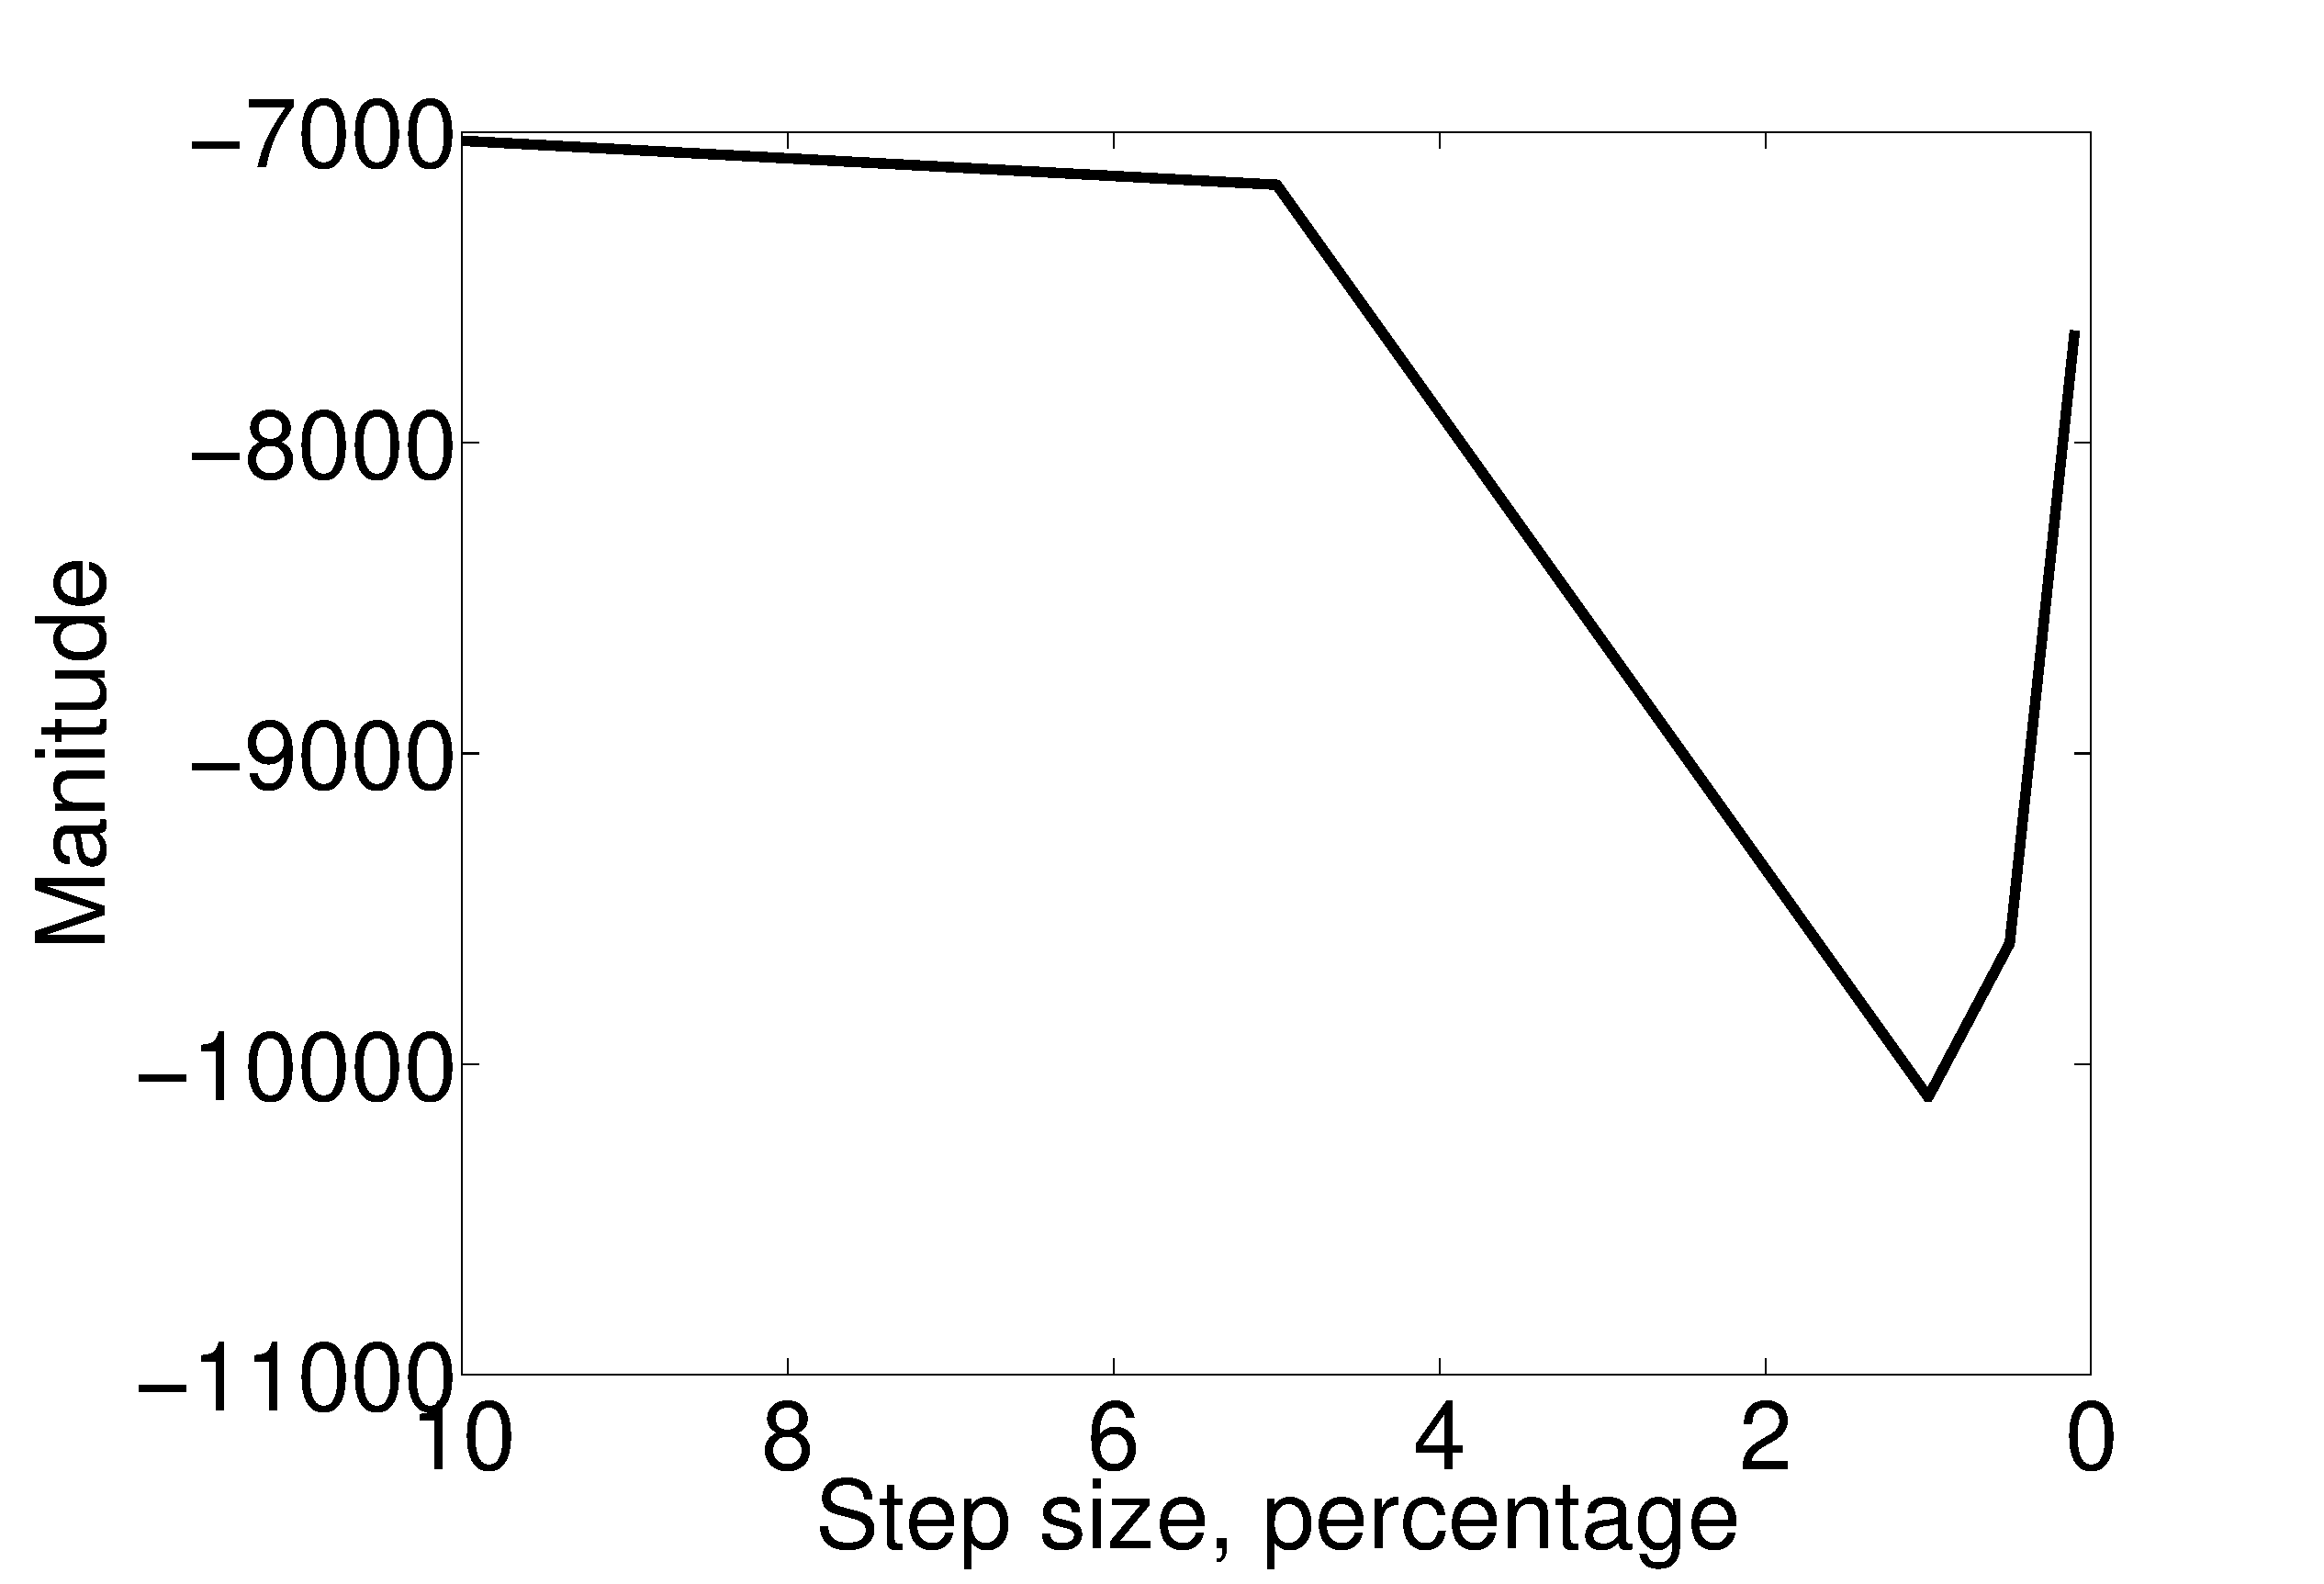
\includegraphics[height=5.15cm]{step_size_4.eps}
		\label{fig:results_hist}
		}
		\\
		\subfigure[Sensitivity with respect to change in length of wing.]
		{
		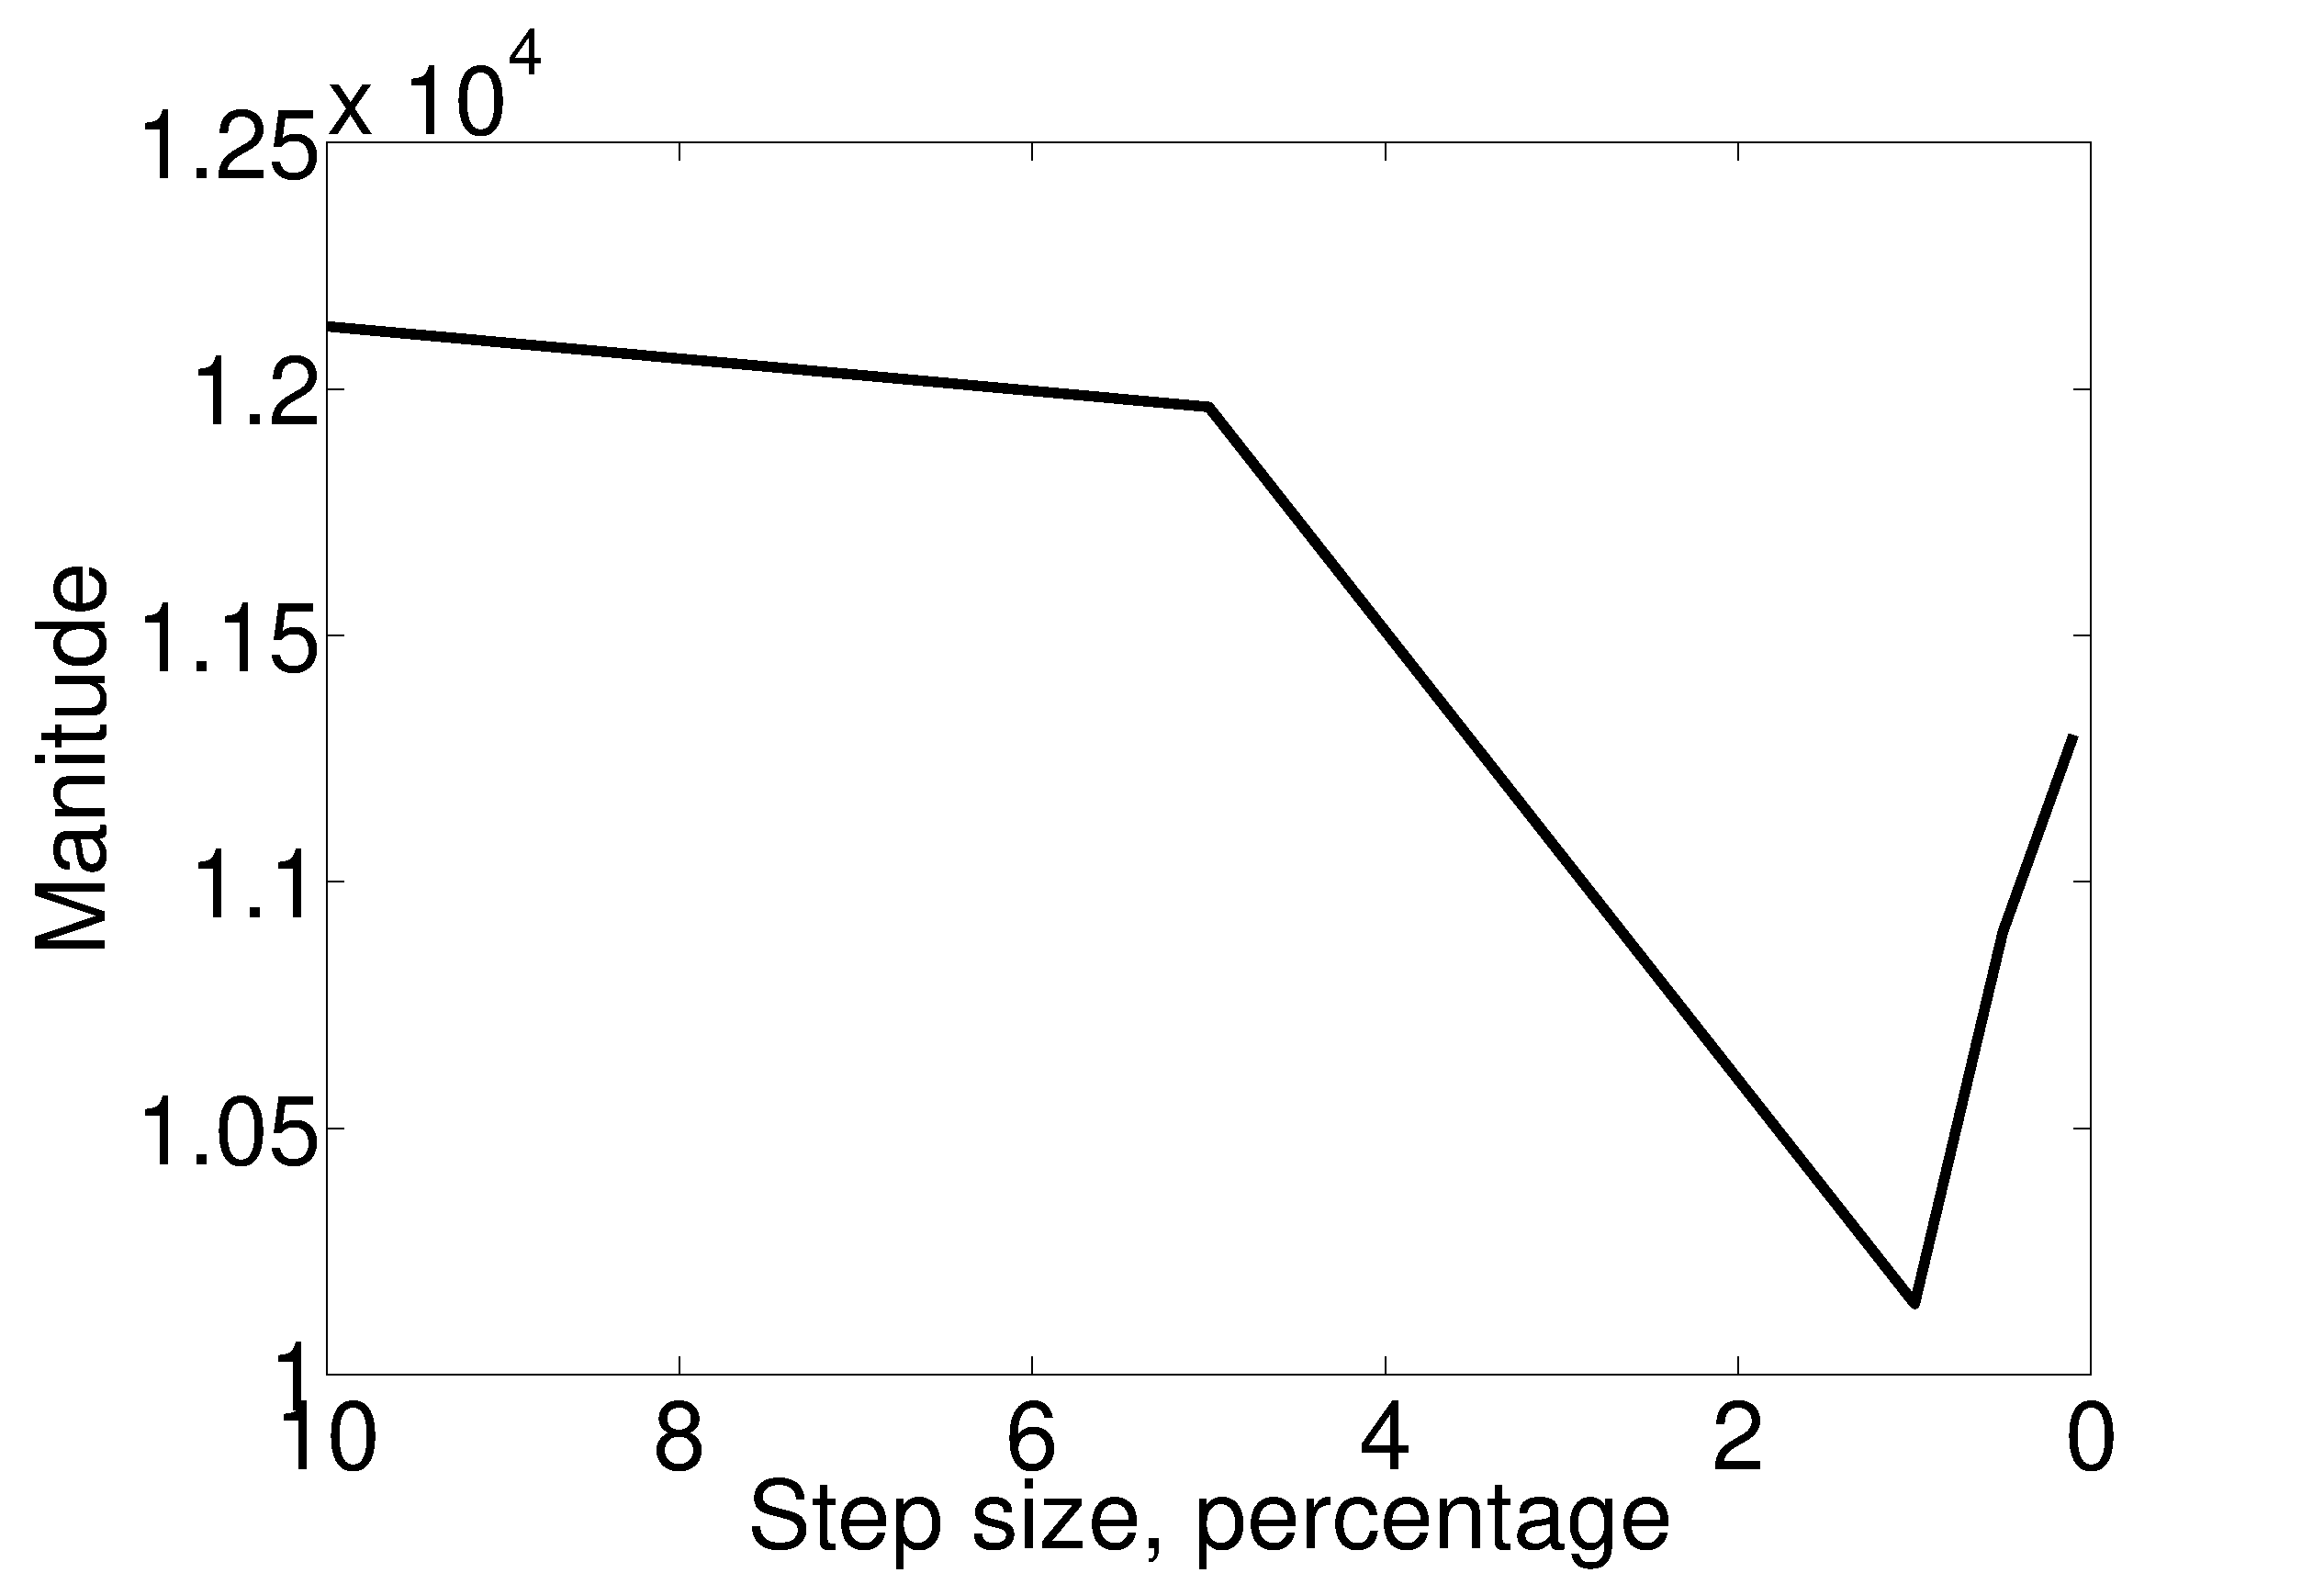
\includegraphics[height=5.15cm]{step_size_5.eps}
		\label{fig:results_fft}
		}
		\quad
		\subfigure[Sensitivity with respect to change in area moment of inertia.]
		{
		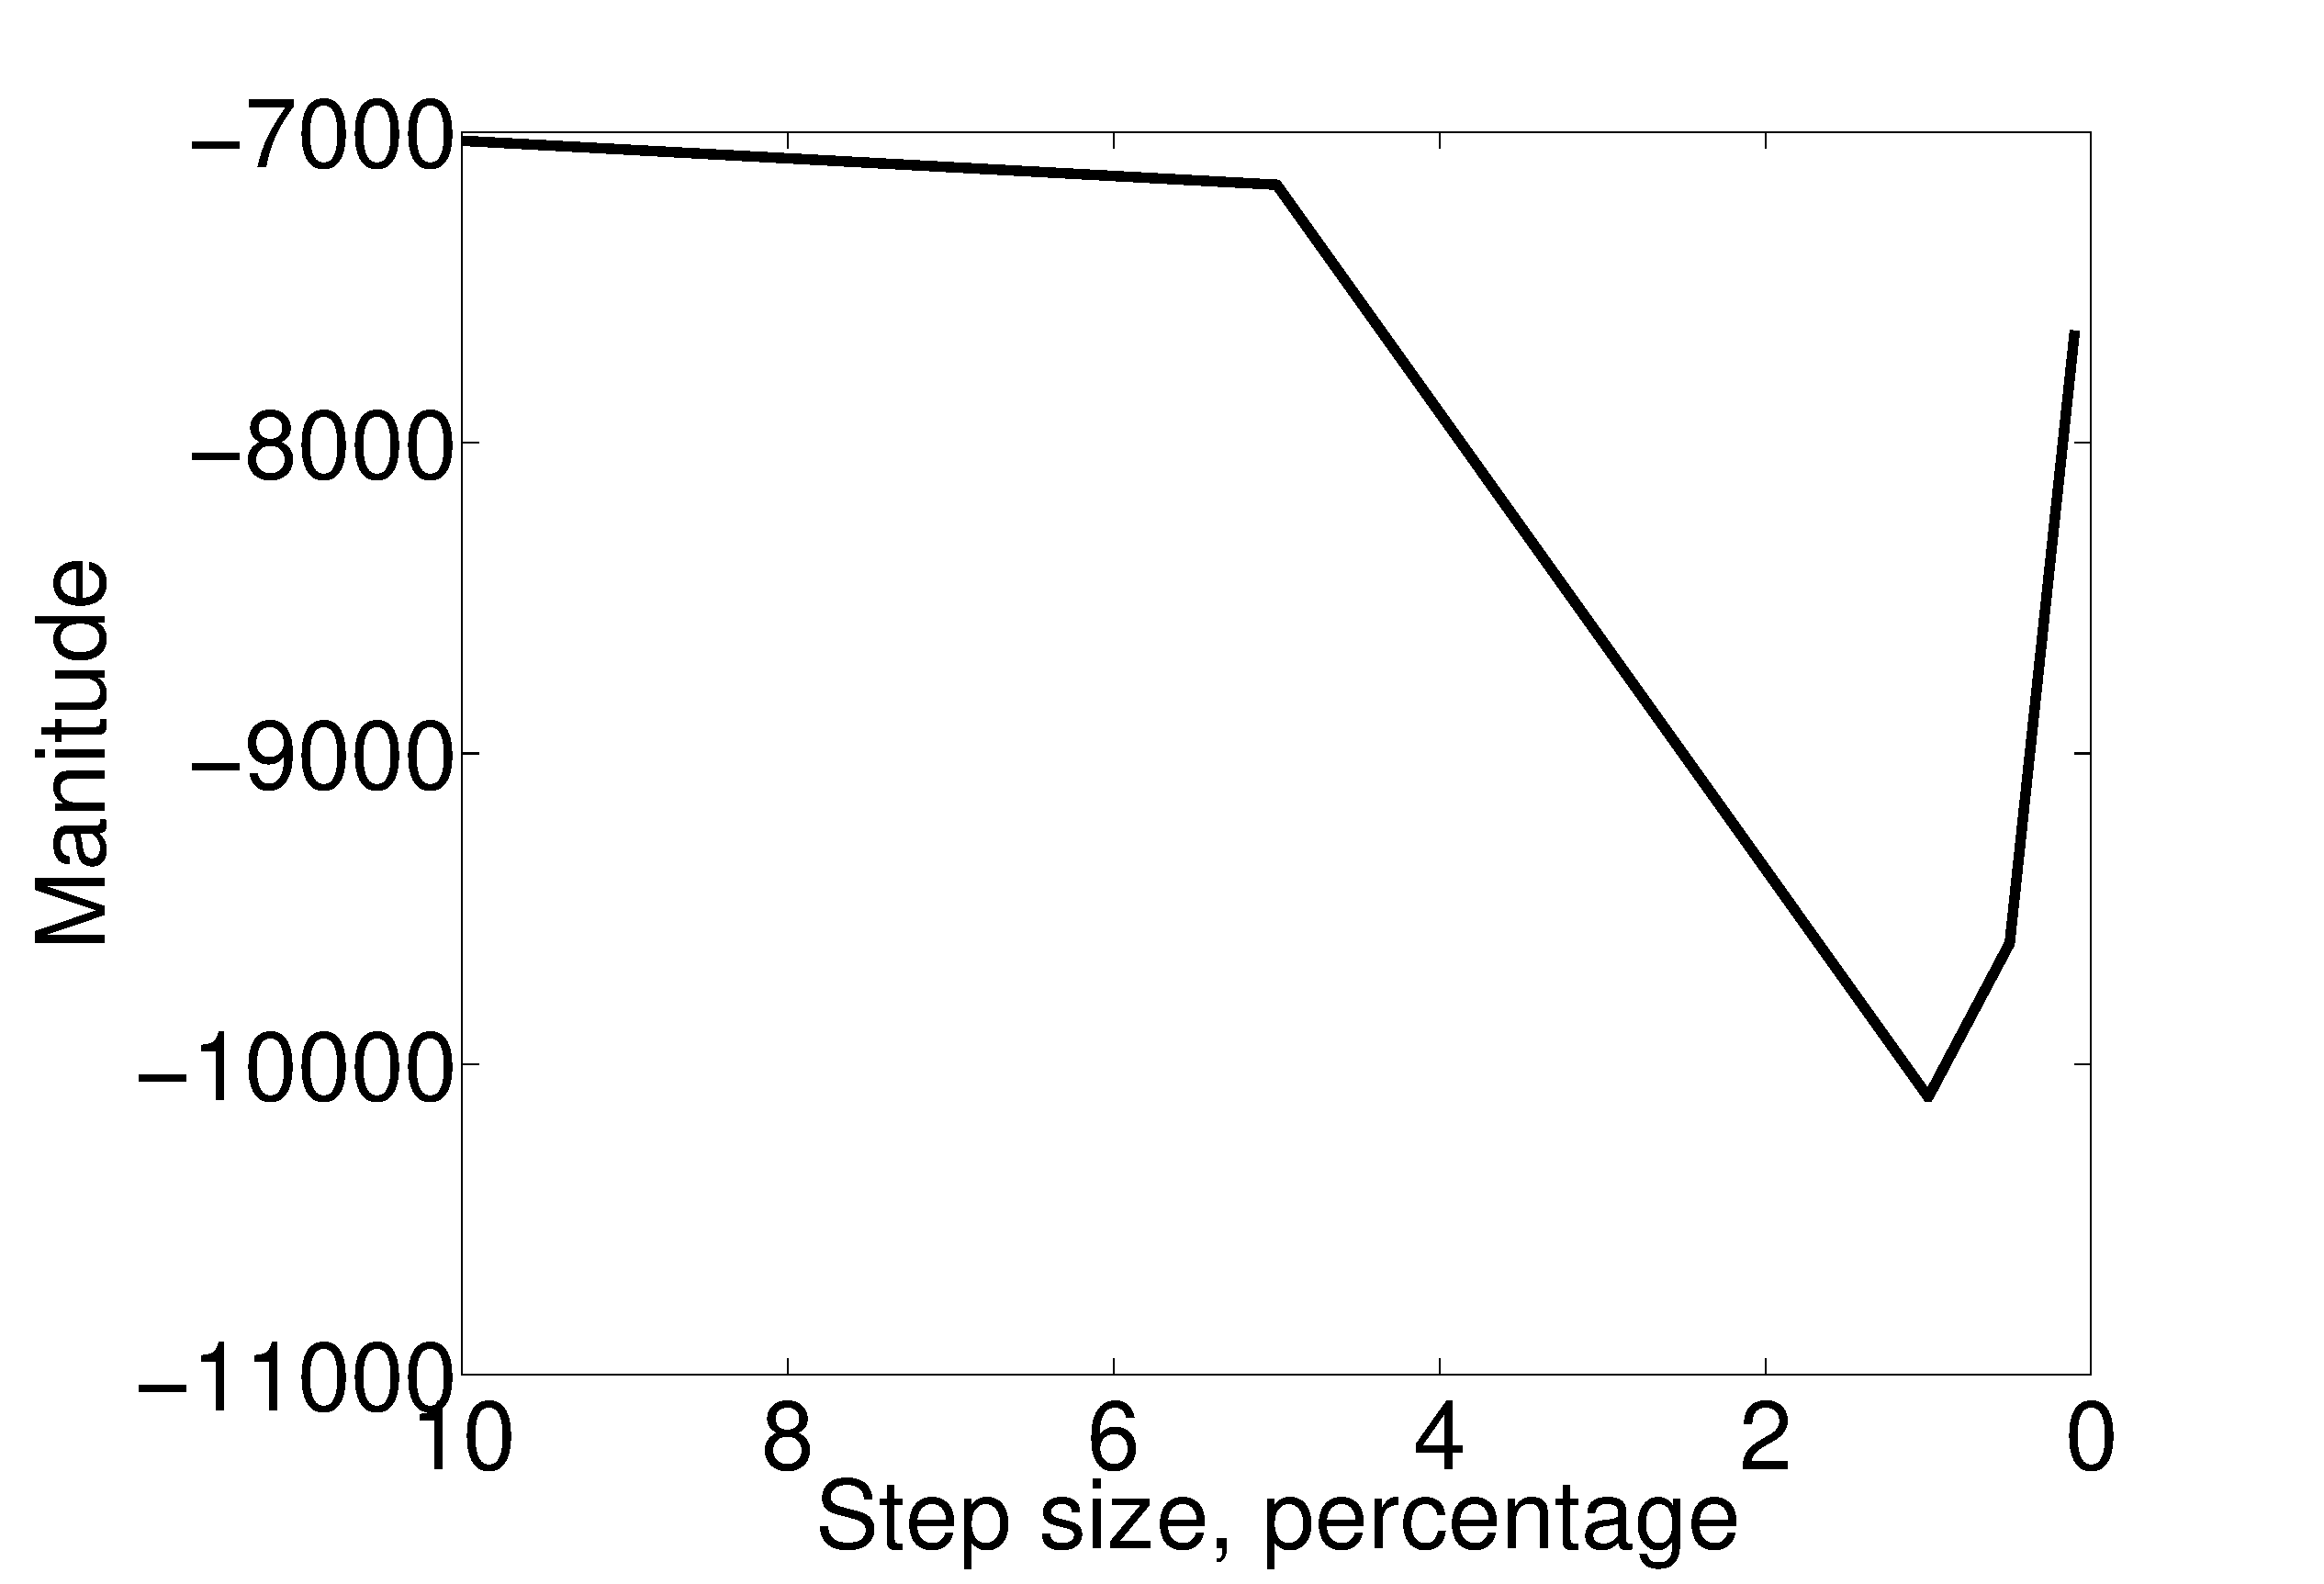
\includegraphics[height=5.15cm]{step_size_6.eps}
		\label{fig:results_hist}
		}
		\caption{Comparison between different step sizes on the sensitivity result.}
		\label{fig:sensitivity_FD_stepsize}
	\end{figure}
%
%----------------------------------------------------------------------------------------
%	PROBLEM 1
%----------------------------------------------------------------------------------------
\section{Solution Approach}\label{sec:solutionApproach}
\subsection{FORM Algorithm Utilizing Approximate Normal Distribution and Adaptive Function Approximation}
There are multiple methods that can be used to calculate the probability of failure for this problem. For sake of clearance, the failure for this problem is defined as the lift force becomes lower than 10,000 N. The lift force is calculated by solving the FSI problem as described in the previous section. In this section, we talk about the reliability methods that are used to calculate the probability of failure.\\

We have used the First Order Reliability Method (FORM) to calculate the reliability index \cite{choi2007reliability}. The problem can be formulated as an optimization problem shown in Equation \eqref{eq:FORM} where $g(U)$ is the limit-state function.
%
\begin{subequations}\label{eq:FORM}
\begin{align}
	\text{Minimize: }& \beta = \sqrt{\left( U^T U \right)}
	\\
	\text{Subject to: }& g \left( U \right) = 0 \quad \text{where} \quad
		g(U) = \text{F}_{\text{LIFT}} - 10000
\end{align}
\end{subequations}
%
The optimization process requires multiple calls to the FSI simulation box to calculate the value of the limit-state function. Since each FSI solution takes approximately 20 minutes to converge this is not feasible. Therefore, a surrogate technique based on two point function approximation (TANA) \cite{wang1995improved} is used as the model the inner loop inside the optimization procedure. The surrogate is then updated at the new point found by the optimizer.\\

TANA requires two points and the gradient information in order to generate the surrogate of the limit-state function. The gradients are calculated using the finite-difference method. The convergence study for the step size in shown in the previous section. In this project, \texttt{calcGrad(X} function is used any time function gradients are needed to be calculated. \texttt{fmincon} is used to calculate the non-linearity index of TANA. The non-linearity index is forced to always be between -3 and 3. High nonlinear indexes will cause the surrogate to have high sensitivities that will produce problems when using gradient based optimization techniques to calculate the safety index.\\

Matlab's \texttt{fmincon} function is used to solve the optimization problem of calculating the reliability index. The optimizer method is chosen as the \emph{Sequential quadratic programming} method for the optimization. SQP method gave us a more steady convergence compared to other methods such as interior-point or active-set. Since the optimizer is working with TANA function approximation and therefore there are no cost of multiple function calls, the tolerances are selected very low. Both tolerances on the constraint satisfaction and design variables are selected as 1E-10.\\

The FORM algorithm requires the random variables to have normal distributions. As pointed out in the previous chapter, the normal distribution is not a valid distribution for many different properties. Therefore, it is needed to calculate the \emph{approximate normal distribution} properties at each design point using Equation \eqref{approximateNormalDistribution} where $F_{x_i}\left( x_i \right)$ is the marginal cumulative distribution function, $f_{x_i}\left( x_i \right)$ is the probability density function, and $\mu_{x_i^\prime}$ and $\sigma_{x_i^\prime}$ are the equivalent means and standard deviations of the approximate normal distributions.
%
\begin{subequations}\label{approximateNormalDistribution}
\begin{align}
\sigma_{x_i^\prime} &= \frac{\phi \left( \Phi^{-1} \left[F_{x_i} \left(x_i^* \right) \right] \right)}{f_{x_i} \left( x_i^* \right)}
\\
\mu_{x_i^\prime} &= x_i^* - \Phi^{-1} \left[ F_{x_i} \left( x_i^* \right) \right] \sigma_{x_i^\prime}
\end{align}
\end{subequations}
%
When using FORM with TANA to calculate the reliability index the starting point is the mean value of the random variables. The second point is calculated using the \emph{Hasofer Line - Rackwitz Fiessler} (HL-RF) method. Using the value of limit-state and its gradients at the second point, TANA surrogate is built. The reliability index at the second point is calculated by solving the optimization problem of Equation \eqref{eq:FORM}. A new surrogate is created at the new point until the convergence criteria is satisfied.
%----------------------------------------------------------------------------------------
\subsection{FFT for Calculating the Probability Distribution Function}
Using the convolution theorem it is possible to get an exact solution of failure probability for the limit-state function. This is valid as long as the limit-state can be defined using a sum of random variables regardless the shape of the distributions. Usually the direct evaluation of the convolution integral for an arbitrary limit-state is not possible. Therefore, the Fast Fourier Transform (FFT) technique is used to evaluate the convolution integral \cite{penmetsa2003adaptation}.\\

In this project we have used TANA as a method to approximate the limit-state function as shown in Equation \eqref{eq:TANA}. 
%
\begin{gather}\label{eq:TANA}
	\tilde{g}(X) = g(X_k) + \frac{1}{r}
	\left[
	x_{i,k}^{(1-r)} \frac{\partial g(X_k)}{\partial x_i} \left( x_i^r - x_{i,k}^r \right)
	\right]
\end{gather}
%
For simplicity, above can be written as:
%
\begin{gather*}
	\tilde{g}(X) = \mathcal{C} + \sum a_i x_i^r
\end{gather*}
%
where
%
\begin{align*}
	\mathcal{C} &= g(X_k) - \frac{1}{r} \sum x_{i,k} \frac{\partial g(X_k)}{\partial x_i}
	\\
	a_i &= \frac{1}{r} x_i^{(1-r)} \frac{\partial g(X_k)}{\partial x_i}
\end{align*}
%
In order to use the convolution theorem to get the limit-state probability distribution, it is needed to write the limit-state in terms of sum of random variables. This is achieved by using the intervening variables $y_i$ as defined in Equation \eqref{eq:interveningVariables}.
%
\begin{subequations}\label{eq:interveningVariables}
\begin{align}
	y_1 &= \mathcal{C} + a_1 x_1^r
	\\
	y_i &= a_i x_i^r \quad , \quad \text{i = 2:n}
\end{align}
\end{subequations}
%
Using the chain rule, the probability density function of the intervening variable $y_i$ is found as shown in Equation \eqref{eq:interveningPDF}. It should be noted that it is necessary to take the absolute value of $\dfrac{dx_i}{dy_i}$ since probability density functions cannot be negative.
%
\begin{gather}\label{eq:interveningPDF}
	f_{y_i} = \left| \frac{dx_i}{dy_i} \right| f_{x_i} \left( x_i \right)
\end{gather}
%
where
%
\begin{subequations}
\begin{align*}
	\frac{dx_1}{dy_1} &= \frac{1}{ra_1} \left( \frac{y_1 - \mathcal{C}}{a_1} 
		\right) ^ \frac{1-r}{r}
	\\
	\frac{dx_i}{dy_i} &= \frac{1}{ra_i} \left( \frac{y_i}{a_i} \right)^\frac{1-r}
		{r} \quad , \quad \text{i = 2:n}
\end{align*}
\end{subequations}
%
Using Equations \eqref{eq:TANA}, \eqref{eq:interveningVariables} and \eqref{eq:interveningPDF} the limit-state function can be written as summation of random variables. Therefore, the PDF of $\tilde{g}$, is the convolution of the individual PDFs of the intervening variables $y_i$ as shown in Equation \eqref{eq:convolutionPDFs}.
%
\begin{gather}\label{eq:convolutionPDFs}
	f_{\tilde{g}} \left( \tilde{g} \right) = f_{y_1} \left( x_1 \right) * f_{y_2}
		\left( x_2 \right) * \dots * f_{y_n} \left( x_n \right)
\end{gather}
%
The bound of the final distribution is calculated by adding the individual intervening variables. This can be written as shown in Equation \eqref{eq:FFTbounds}.
%
\begin{subequations}\label{eq:FFTbounds}
\begin{align}
	\tilde{g}^{\text{min}} = \sum y_i^{\text{min}}
	\\
	\tilde{g}^{\text{max}} = \sum y_i^{\text{max}}
\end{align}
\end{subequations}
%
The probability of failure can then be calculated as
%
\begin{gather}
	p_f = \int_{\tilde{g}^{\text{min}}}^0 f_{\tilde{g}} d\tilde{g}
\end{gather}
%
%----------------------------------------------------------------------------------------
%	PROBLEM 1
%----------------------------------------------------------------------------------------
\section{Results and Discussion}
%----------------------------------------------------------------------------------------
\subsection{FORM Results}
As discussed in Section ~\ref{sec:solutionApproach}, FORM with adaptive function approximation (TANA) is used to calculate the reliability index. Since some of the variables had non-normal distributions, approximate normal distribution is calculated for each of random variables at each of the design points. The results of FORM algorithm is shown in Tables ~\ref{table:resultsFORM_eqNormal} and ~\ref{table:resultsFORM_Normal}. Table ~\ref{table:resultsFORM_eqNormal} contains the results based on non-normal distribution of random variables whereas ~\ref{table:resultsFORM_Normal} is the data assuming every variable has normal distribution with same mean as non-normal distributions. The probability of failure of the first case (variables with non-normal distributions) is \textbf{0.95\%} and for the second case (variables with non-normal distributions) is \textbf{2.35\%}. These two values are close to each other as expected.
%
\begin{table}[H]
\centering
\begin{tabular}{ c || c | c | c | c }
	Iteration Number & 1 & 2 & 3 & 4 \\
	\hline
	U & 265 & 237.85 & 237.03 & 220.39 \\
	$\alpha$ & 0.1 & 5.7656 & 4.9503 & 4.4867 \\
	$C_0$ & 0.5 & 0.49039 & 0.51206 & 0.50139 \\
	E & 2.00E+11 & 1.93E+11 & 1.93E+11 & 1.93E+11 \\
	L & 1 & 0.97544 & 0.84538 & 0.97244 \\
	I & 5.20E-07 & 5.22E-07 & 6.26E-07 & 5.13E-07 \\
	dg/dU & 49743.8 & 45118.9 & 28837.3 & 36411 \\
	dg/d$\alpha$ & 159.65 & 229.57 & 361.8 & 669.59 \\
	dg/d$C_0$ & -480.8 & -366.52 & -278.77 & -267.72 \\
	dg/dE & -7132 & -6366.6 & -6117 & -2696.8 \\
	dg/dL & 12630 & 9741.9 & 2224.6 & 1134.2 \\
	dg/dI & -7091.2 & -6139.12 & -4914.26 & -2645.812 \\
	g & 1232.8 & 2898.2 & 627.34 & 0.35 \\
	r & 0 & 3 & 2.35 & 2.37 \\
	$\beta$ & 0.99995 & 4.3521 & 1.6322 & 2.342 \\
	$\epsilon$ & 1 & 0.64272 & 0.71479 & 0.00735 \\
	\hline
\end{tabular}
\caption{FORM convergence history with non-normal variables.}
\label{table:resultsFORM_eqNormal}
\end{table}
%
%
\begin{table}[H]
\centering
\begin{tabular}{ c || c | c | c | c }
	Iteration Number & 1 & 2 & 3 & 4 \\
	\hline
	Iteration Number & 1 & 2 & 3 & 4 \\
	U & 265 & 247.65 & 256.12 & 237.04 \\
	$\alpha$ & 0.1 & 4.6327 & 4.0544 & 3.8588 \\
	$C_0$ & 0.5 & 0.50065 & 0.49794 & 0.50355 \\
	E & 2.00E+11 & 2.01E+11 & 2.01E+11 & 2.01E+11 \\
	L & 1 & 0.99262 & 1.0259 & 1.0233 \\
	I & 5.20E-07 & 5.61E-07 & 5.27E-07 & 4.70E-07 \\
	dg/dU & 49743.8 & 13312.01 & 49093.9 & 25329.76 \\
	dg/d$\alpha$ & 159.65 & 8668.9 & 1133.5 & 5132 \\
	dg/d$C_0$ & -480.8 & -135.24 & -653.42 & -479.35 \\
	dg/dE & -7132 & -29192 & -15339 & -15857 \\
	dg/dL & 12630 & 6752.6 & 13148 & 6190.7 \\
	dg/dI & -7091.2 & -27357.2 & -15175.68 & -17628.52 \\
	g & 1232.8 & 2923.9 & 732.4 & 0.73 \\
	r & 0 & 3 & 2.12 & 2.43 \\
	$\beta$ & 0.93372 & 0.8449 & 1.3416 & 1.985 \\
	$\epsilon$ & 1 & 0.10512 & 0.37023 & 0.12218 \\
	\hline
\end{tabular}
\caption{FORM convergence history with normal variables.}
\label{table:resultsFORM_Normal}
\end{table}
%
%----------------------------------------------------------------------------------------
\subsection{FFT Results}
As discussed in Section ~\ref{sec:solutionApproach}, using TANA and intervening variables, the limit-state function can be written as summation of random variables. Therefore, the limit-state probability density function is the convolution of the PDFs of each random variable. The most efficient way of calculating this convolution is to use the Fast Fourier Transform (FFT) to transfer the probabilities to the frequency domain. In frequency domain, convolution is done by multiplying the function. This result needs to be transformed back into the original form using inverse Fourier transforms.\\

In this project, Matlab's \texttt{fft} function is used to calculate the Fourier transform of the probability density functions. \texttt{fft(X)} works the best if the length of the vector \texttt{X} is equal to a power of 2, i.e. $2^10$. Therefore, the original vectors are \emph{zero padded} to increase their length. After zero padding and calculating the fast Fourier transform of the PDF vector of each random variable, they are multiplied. Inverse Fourier transform is applied on the final result to transfer it back to the original form. The bounds are calculated from Equation \eqref{eq:FFTbounds}. The surrogate bounds are calculated as -8704.2 and 2.6114E+5. The probability density function of the limit-state is shown in Figure ~\ref{fig:FFT_result}. The probability of failure is calculated from the PDF plot is \textbf{0.26\%}. This is close to the value calculated using FORM algorithm with non-normal distributions.\\

As discussed in Section ~\ref{sec:solutionApproach}, TANA approximation is used to write the limit-state as summation of the random variables. One of the reasons that the $p_f$ result from FFT does not matches the FORM solution can be related to the approximation used to represent the limit-state as summation of random variables. Higher-order approximation methods such as TANA2 can be used to improve the accuracy of the results. TANA2 can replace the function approximation in the optimization loop of FORM algorithm and also the approximation used in FFT method as is shown in Equation \eqref{eq:TANA}.
%
\begin{figure}[H]
	\centering
	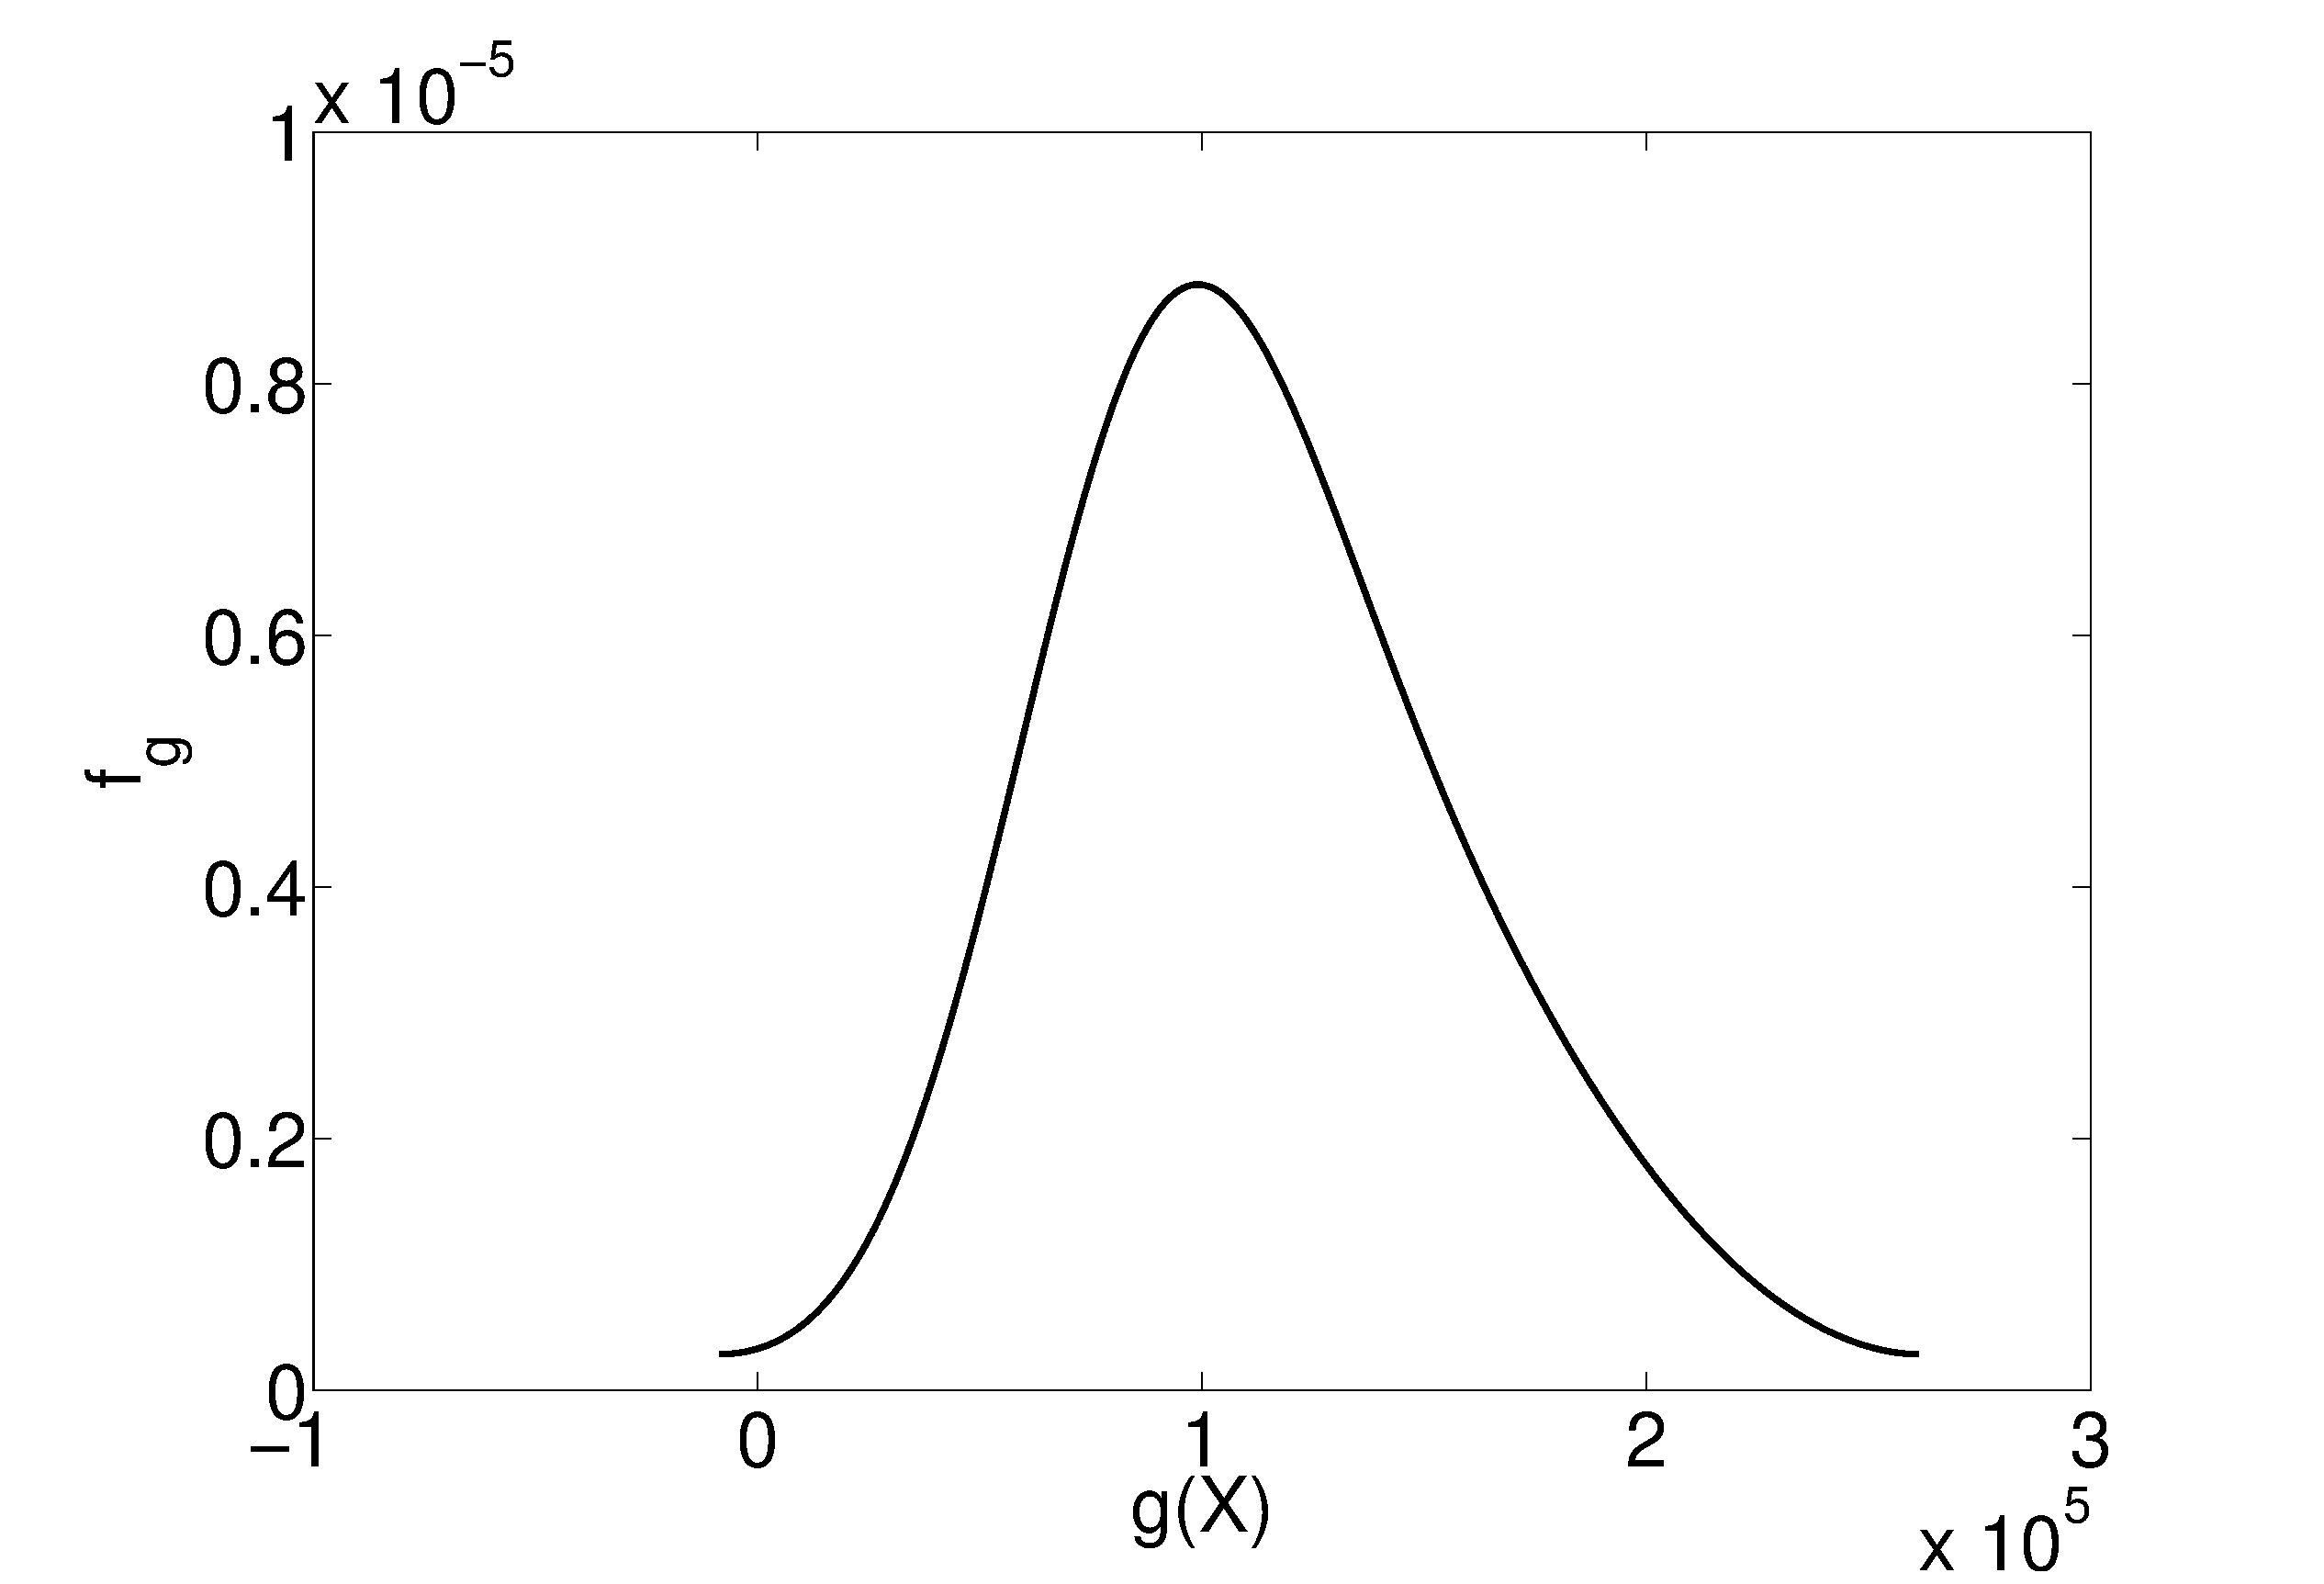
\includegraphics[height=7.5cm]{FFT.eps}
	\caption{Limit-state PDF using FFT.}
	\label{fig:FFT_result}
\end{figure}
%
%----------------------------------------------------------------------------------------
%	PROBLEM 1
%----------------------------------------------------------------------------------------
\section{Summary}
In this project a FSI solver is developed by coupling the solution of a CFD and FEA solver and iterating between them. Matlab is used as an interface for transferring the load and deformation data between the solvers and updating the models. To ensure the stability of the solution, the FEA results are relaxed and then used to update the CFD model. This is especially helpful when the forces coming from the CFD solver cause large deformations in the structure. One of situation where the FSI simulation is needed is in the design of aircraft wings. Therefore, a simplified model of aircraft wing is used as the problem of interest for this project. The wing box is modeled as a single beam element where the lifting surfaces are modeled as an airfoil connected to the tip of the beam. Since the main function of the wing is to generate lift, the limit-state is selected as the generated lift force.\\

Several uncertain variables are selected for this problem. Sensitivity of the limit-state function to uncertain variables is checked to assure their contribution to the limit-state function. Two different reliability methods are used to calculate the probability of failure. FORM is performed with non-normal and normal random variables using two-point adaptive function approximation. It is shown that the two results are close to each other. Moreover, convolution theory is used to derive the PDF of the limit-state function and its probability of failure. By comparing the convolution theory and FORM results it can be seen that the two are close. The difference can be qualified due to the approximation used for writing the limit-state function as a summation of random variables.\\

Observing the probability of failure it can be concluded that the reliability analysis is needed for this problem. Usually for aircraft the probability of failure needs to be much lower than what is calculated in the project. This can be improved by chaining the wing geometry to lower the deflection or redesign the lifting surfaces to generate more lift at the deflected configuration of the wing. The latter is referred to \emph{aeroelastic tailoring}.
%----------------------------------------------------------------------------------------
%	References #
%----------------------------------------------------------------------------------------
\bibliographystyle{aiaa}  
\bibliography{ref}
% ---------------------------------------------------------------------------- %
\end{document}